

\chapter{Binární regrese - klasifikace}
\label{sec:BinarniRegrese}

\par{??????????????}













%------------KLASIFIKACE---------------------------------------------------------
\section{Klasifikace}
\label{sec:BinarniRegreseKlasifikace}

\par{Na úvod si uveďme několik klasifikačních příkladů:
\begin{center}
	\textbf{Spam:} je spam / není spam ?\\
	\textbf{Online transakce:} podvodné ano / ne ?\\
	\textbf{Nádor:} zhoubný / nezhoubný?
\end{center}
Z příkladů je zřejmé, že se jedná o rozhodnutí mezi dvěma možnostmi, tedy $y \in \{ 0, 1 \}$, kde $0$ je \uv{negativní třída} (nezhoubný nádor) a~$1$ je pozitivní třída (zhoubný nádor). Pokud máme $y \in \{ 0, 1 \}$ jedná se o~klasifikaci do dvou tříd, dále existuje klasifikace do více tříd, kde $y \in \{ 0, 1, 2, 3, \ldots \}$. V následujících kapitolách se budeme zabývat klasifikací do dvou tříd.}
\par{Nyní se dostáváme k problému jak vyvinout klasifikační algoritmus, což si můžeme ukázat na příkladu trénovací sady pro úlohu klasifikace nádorů. Nádor může být buď zhoubný nebo nezhoubný, tedy buďto 1 nebo 0. Dostupná data pro náš příklad jsou na obrázku \ref{fig:nadory1}.
\begin{figure}[!ht]
	\centering
	%trim option's parameter order: left bottom right top
	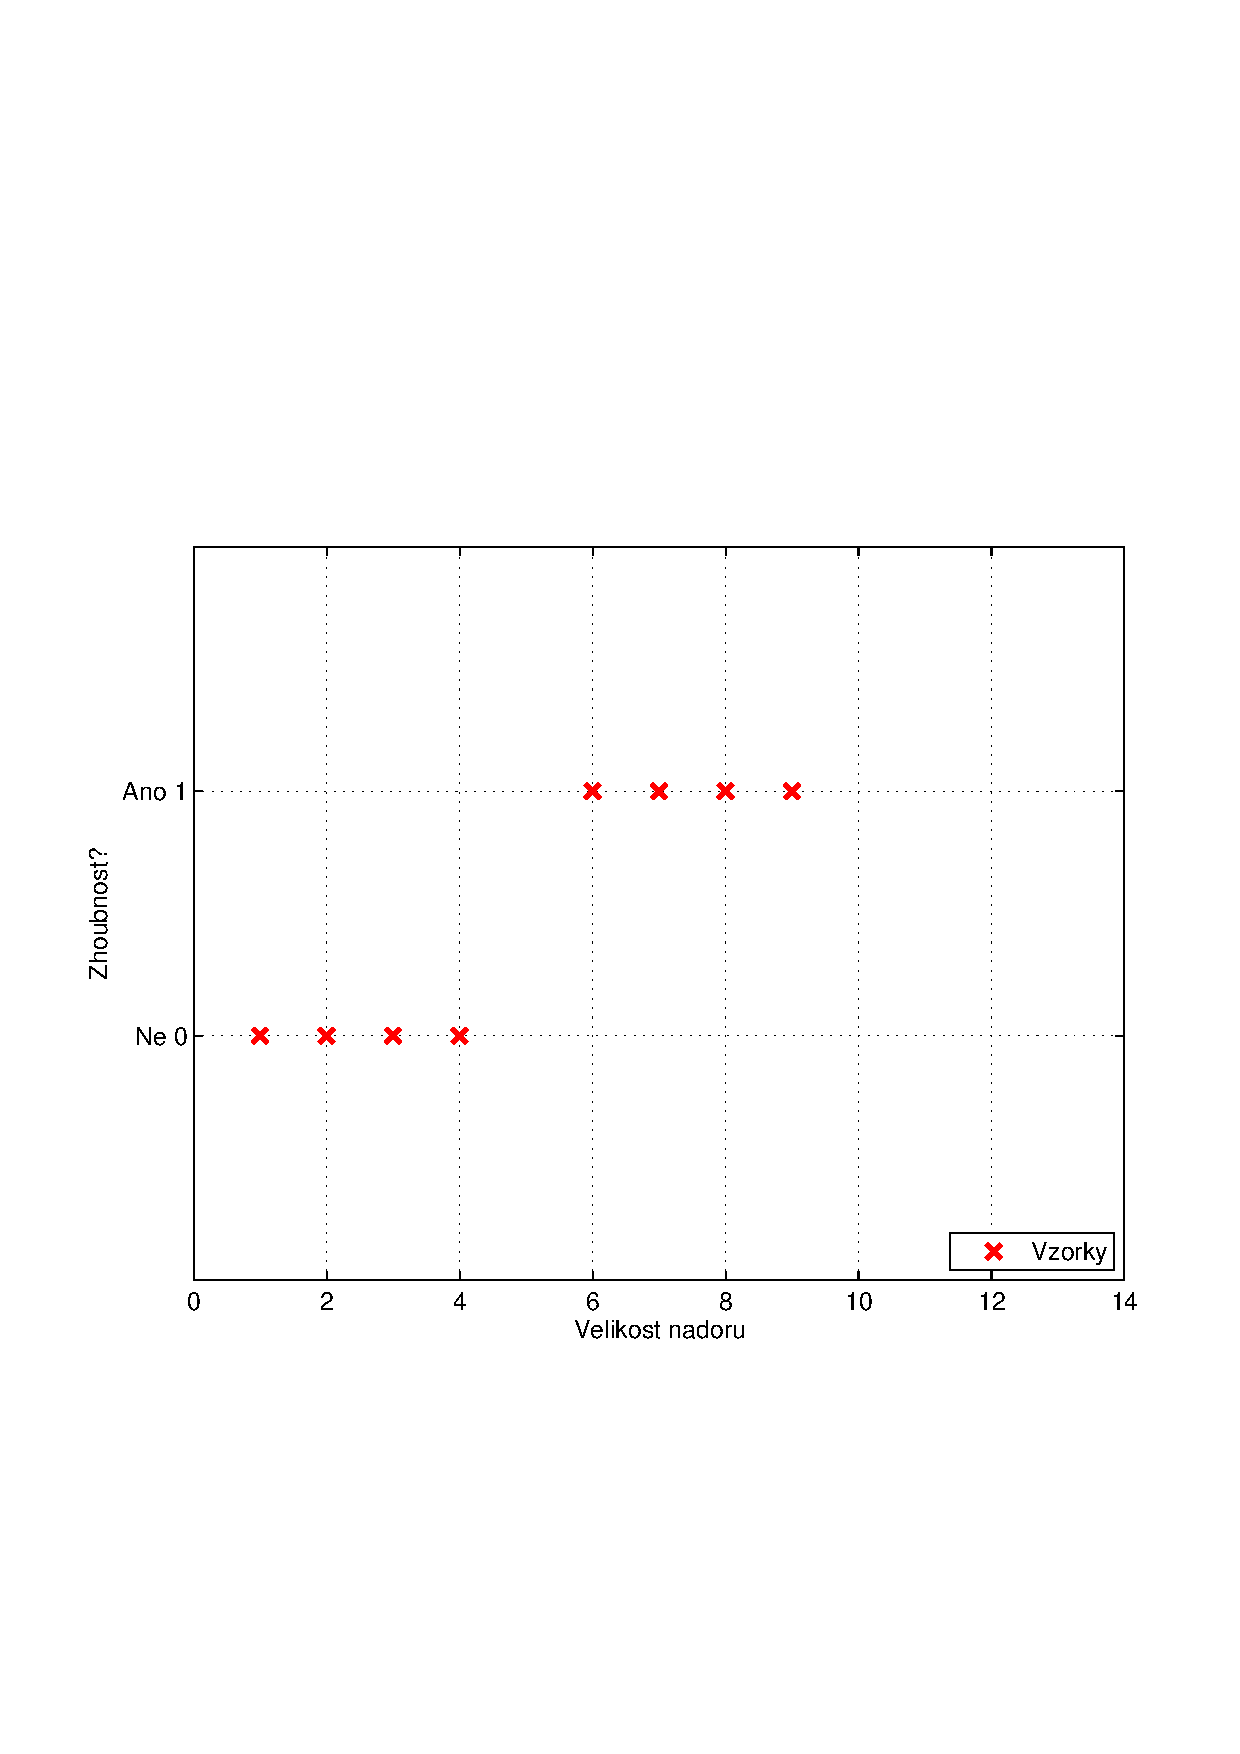
\includegraphics[width = 0.48\textwidth, trim = 2.5cm 7cm 2cm 9cm]{./Img/BinarniRegrese/prikladNadory/tumor_1st_example.pdf}
	\caption{Trénovací data.}
	\label{fig:nadory1}
\end{figure}}
\pagebreak

\par{Jedna z~věcí, kterou bychom mohli udělat, je aplikace algoritmu lineární regrese, který známe z~kapitoly \ref{sec:LinearniRegrese}. Výsledek aplikace hypotézy
\begin{equation}
	h_{\bm{\Theta}} \left( \bm{x} \right) = \bm{\Theta}^{\top} \bm{x}
\end{equation}
lze vidět na Obr. \ref{fig:nadory2}.}

\par{Pokud bychom chtěli udělat predikci ze získané hypotézy, tak můžeme využít klasifikátoru na základě prahování. Tedy hodnotu po jejíž překročení vzorek spadá již do druhé třídy, v~případě binární regrese je to hodnota 0.5. Chceme tedy určit
\begin{eqnarray}
	\label{eq:prah1}
	h_{\bm{\Theta}} \left( \bm{x} \right) \geq 0.5, \quad \mathrm{predikuj~} y = 1,\\
	\label{eq:prah2}
	h_{\bm{\Theta}} \left( \bm{x} \right) < 0.5, \quad \mathrm{predikuj~} y = 0.
\end{eqnarray}
Tento poznatek je reprezentován na Obr. \ref{fig:nadory3}.

\begin{figure}[!ht]
	\centering
	\begin{minipage}[b]{0.48\textwidth}
		%trim option's parameter order: left bottom right top
		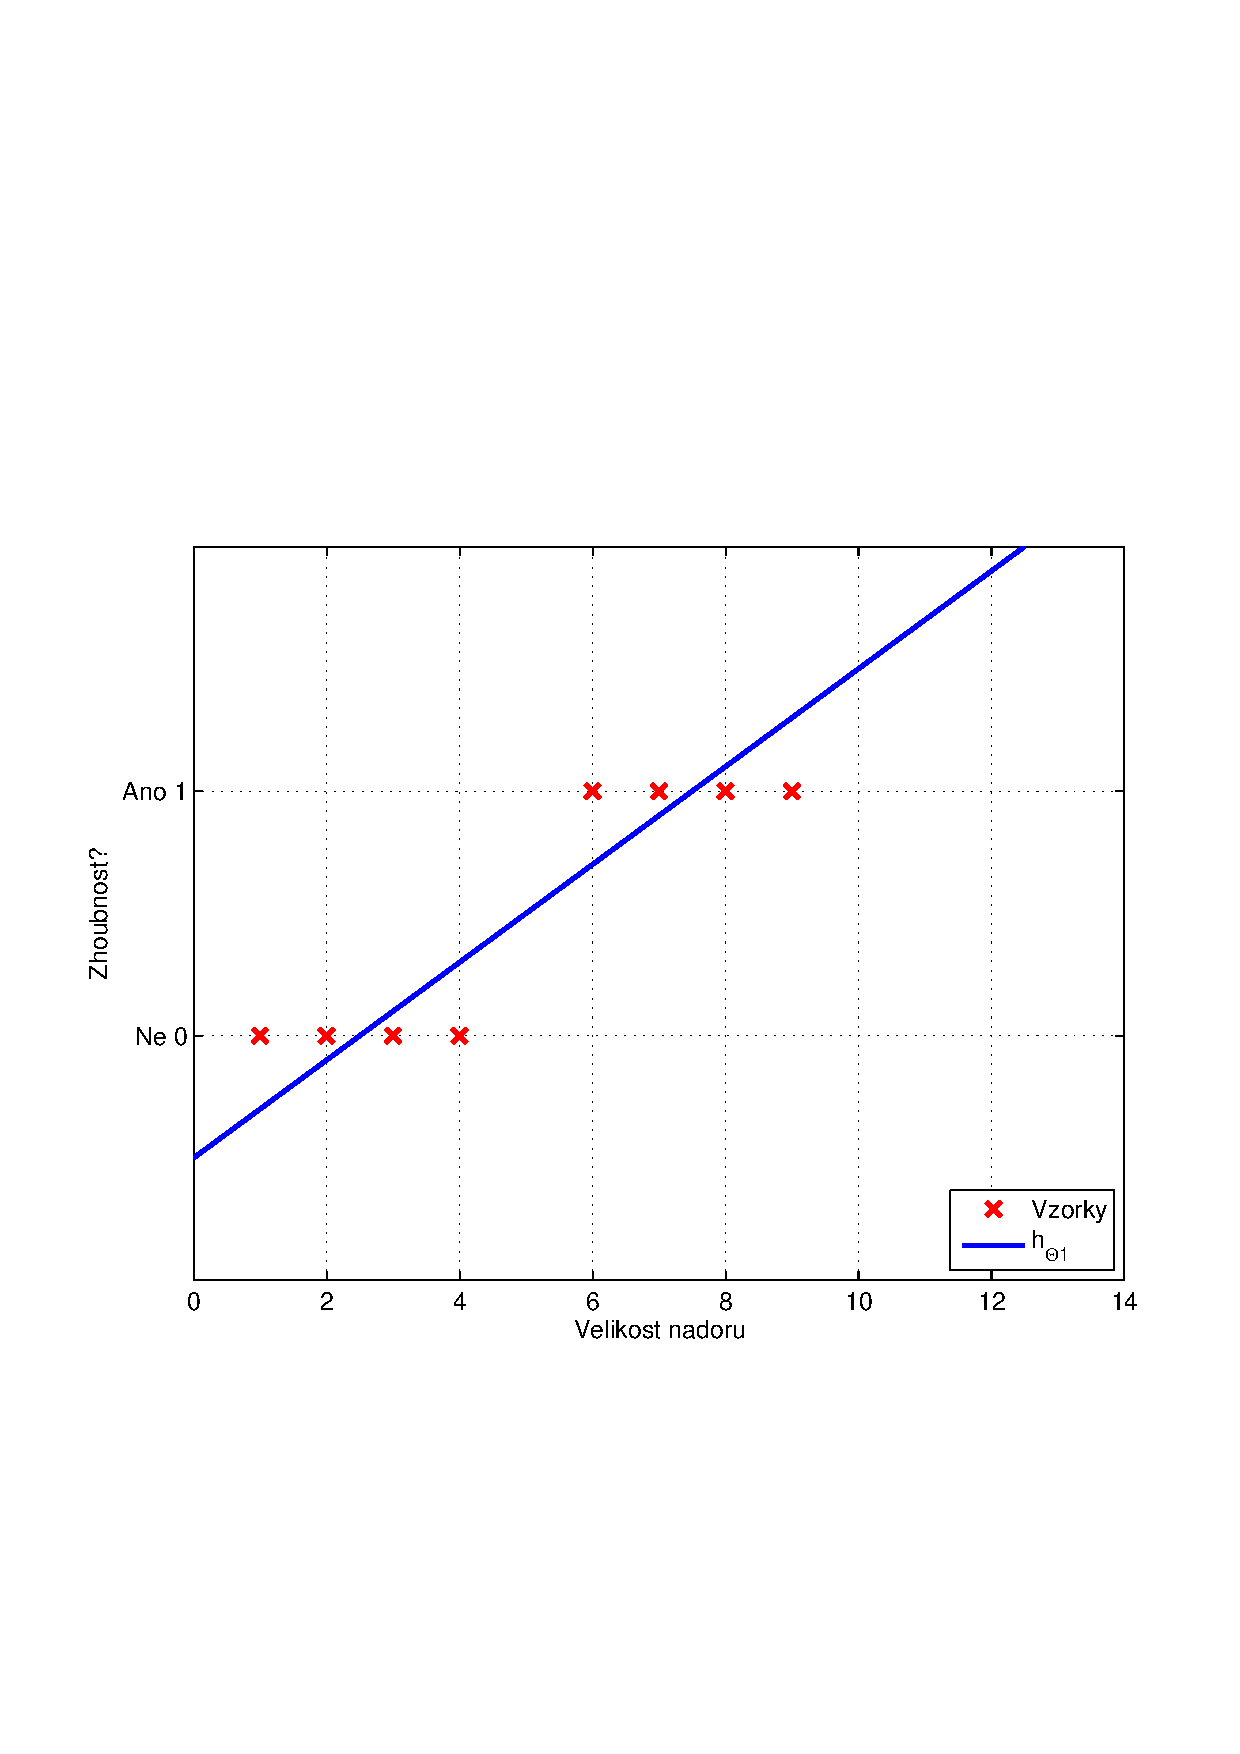
\includegraphics[width = \textwidth, trim = 2.5cm 7cm 2cm 9cm]{./Img/BinarniRegrese/prikladNadory/tumor_2st_example.pdf}
		\caption{Lineární regrese. \\ ~}
		\label{fig:nadory2}
	\end{minipage}%
	\hfill
	\begin{minipage}[b]{0.48\textwidth}
		%trim option's parameter order: left bottom right top
		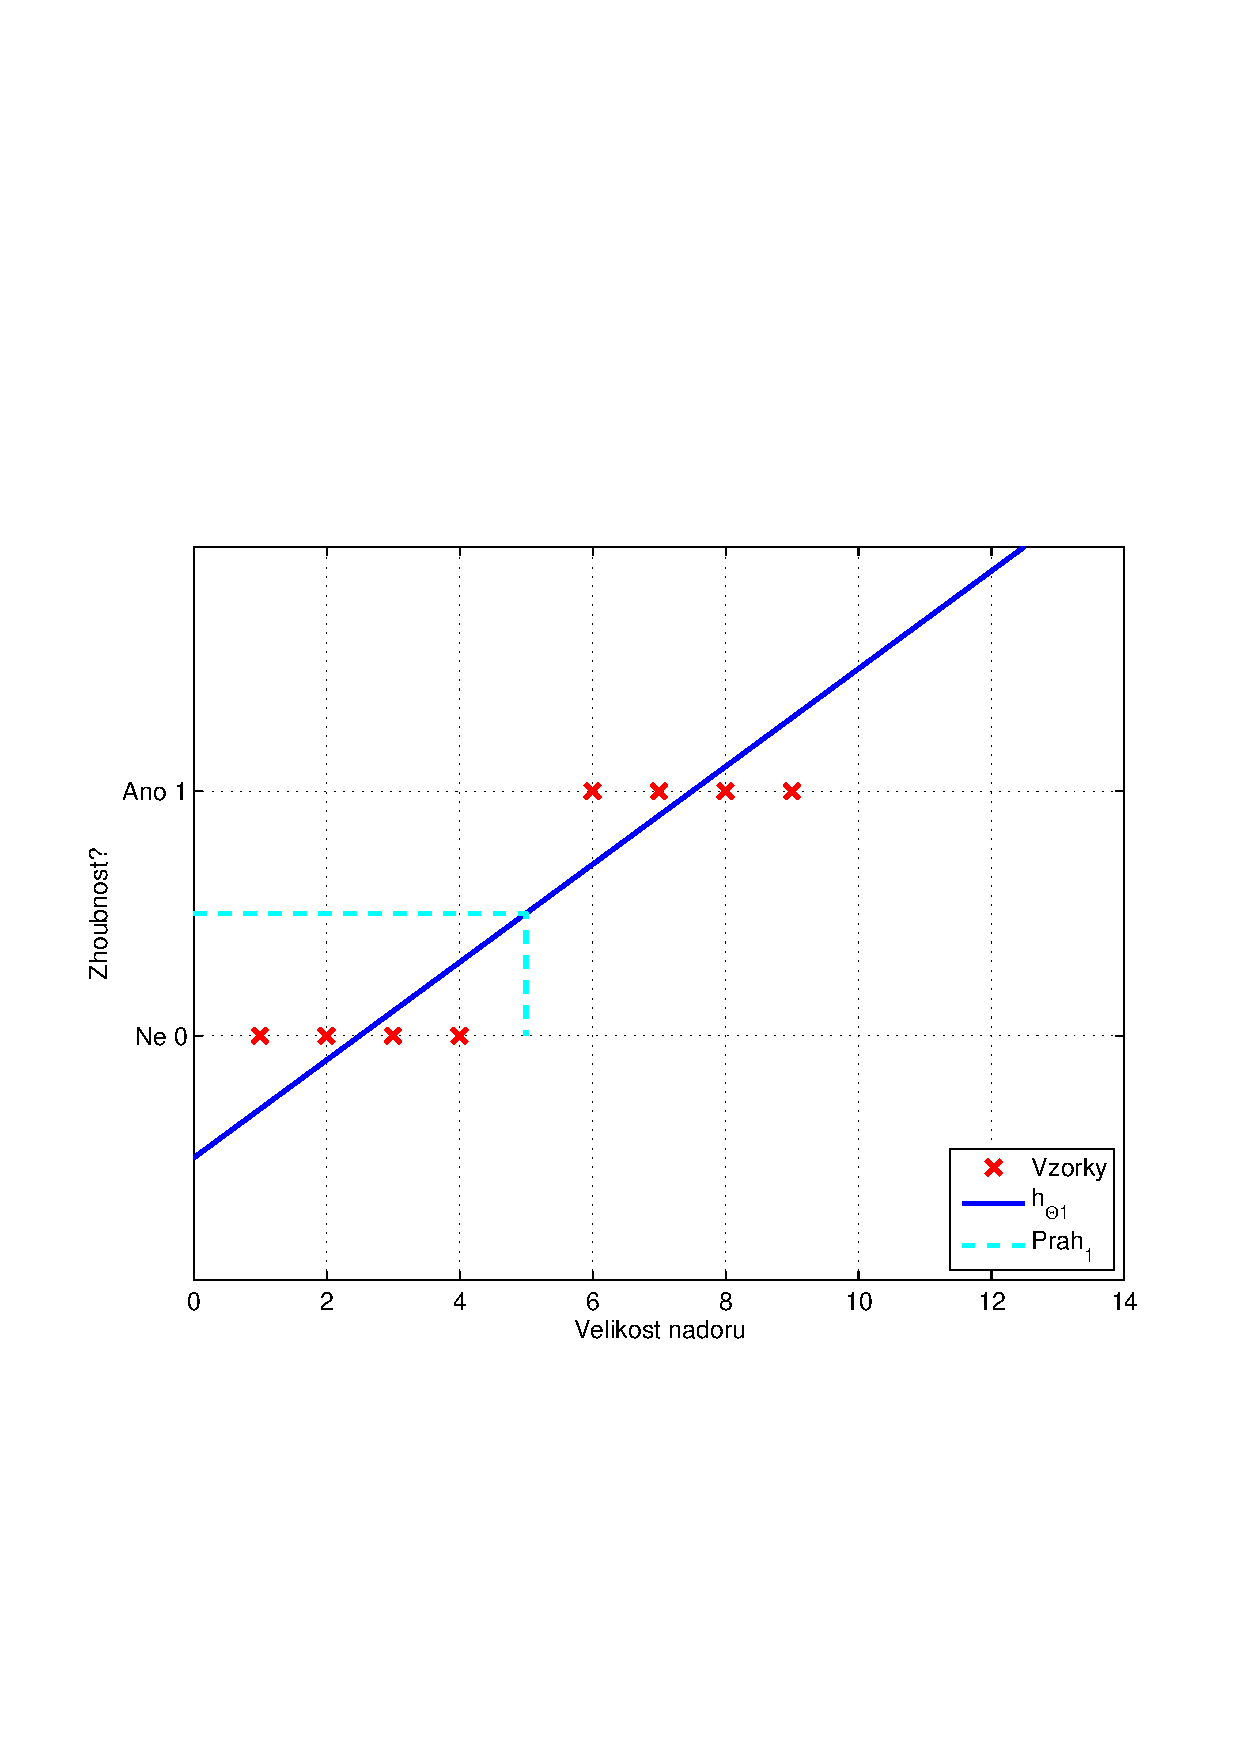
\includegraphics[width = \textwidth, trim = 2.5cm 7cm 2cm 9cm]{./Img/BinarniRegrese/prikladNadory/tumor_3st_example.pdf}
		\caption{Lineární regrese - určení rozhodovacího prahu.}
		\label{fig:nadory3}
	\end{minipage}%
\end{figure}}

\par{V tomto příkladě jsme si ukázali, že lineární regrese dělá něco co by se dalo považovat za řešení klasifikačního problému. Na následujícím rozšíření našeho příkladu bude ukázáno, že tomu tak není.}

\par{Rozšíříme náš příklad o~další vzorky viz Obr. \ref{fig:nadory4}, kde nám přibyly dva vzorky více vpravo. Po aplikování lineární regrese, na rozšířená data, získáváme výsledek, který lze vidět na Obr. \ref{fig:nadory5}. Aktuální hypotéza $h_{\bm{\Theta} 2}$ již nesplňuje podmínky definované vztahy \ref{eq:prah1} a~\ref{eq:prah2}, jelikož první vzorek, který má být vyhodnocen jako zhoubný by v tomto případě byl vyhodnocen jako nezhoubný, což může zásadně ovlivnit něčí život.

\begin{figure}[!ht]
	\centering
	\begin{minipage}[b]{0.48\textwidth}
		%trim option's parameter order: left bottom right top
		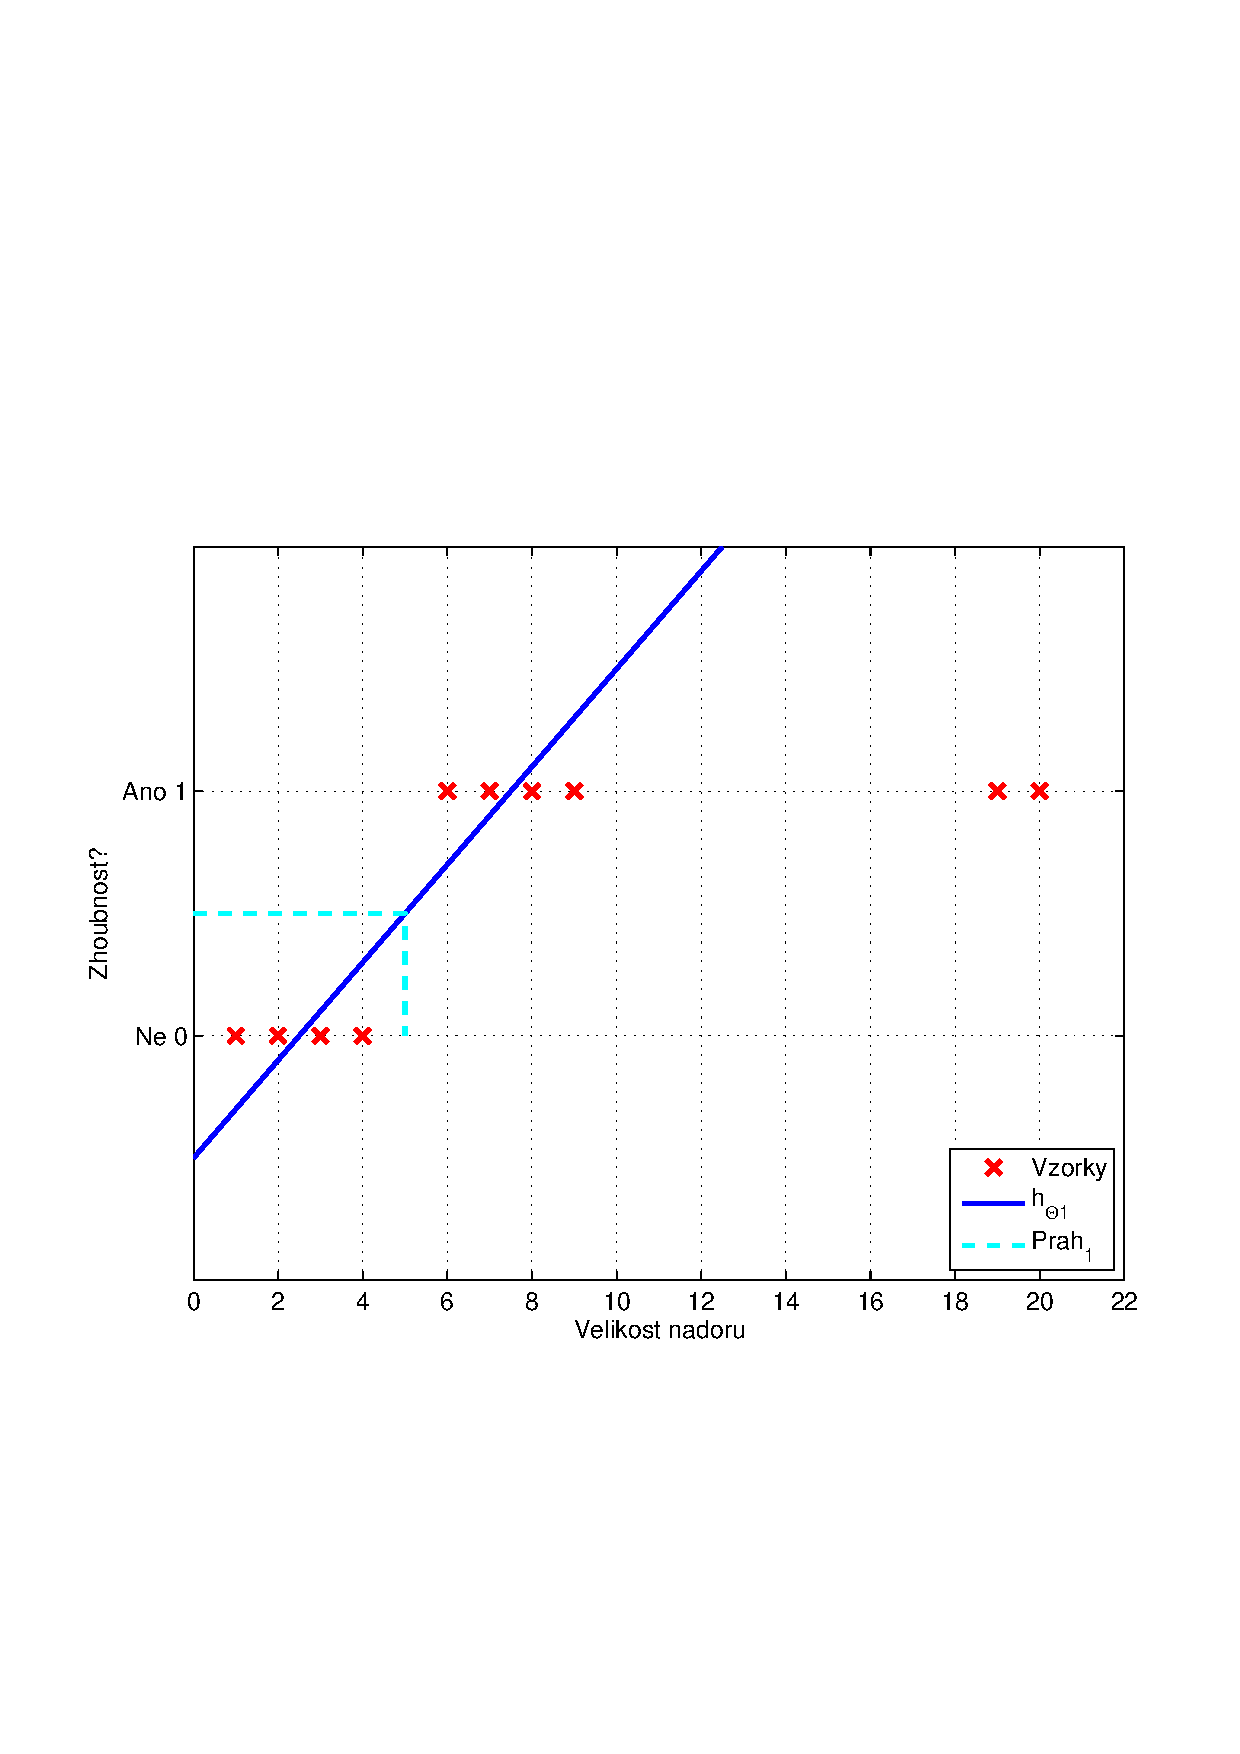
\includegraphics[width = \textwidth, trim = 2.5cm 7cm 2cm 9cm]{./Img/BinarniRegrese/prikladNadory/tumor_4st_example.pdf}
		\caption{Rozšíření trénovací množiny dat o dva vzorky vpravo. \\ ~}
		\label{fig:nadory4}
	\end{minipage}%
	\hfill
	\begin{minipage}[b]{0.48\textwidth}
		%trim option's parameter order: left bottom right top
		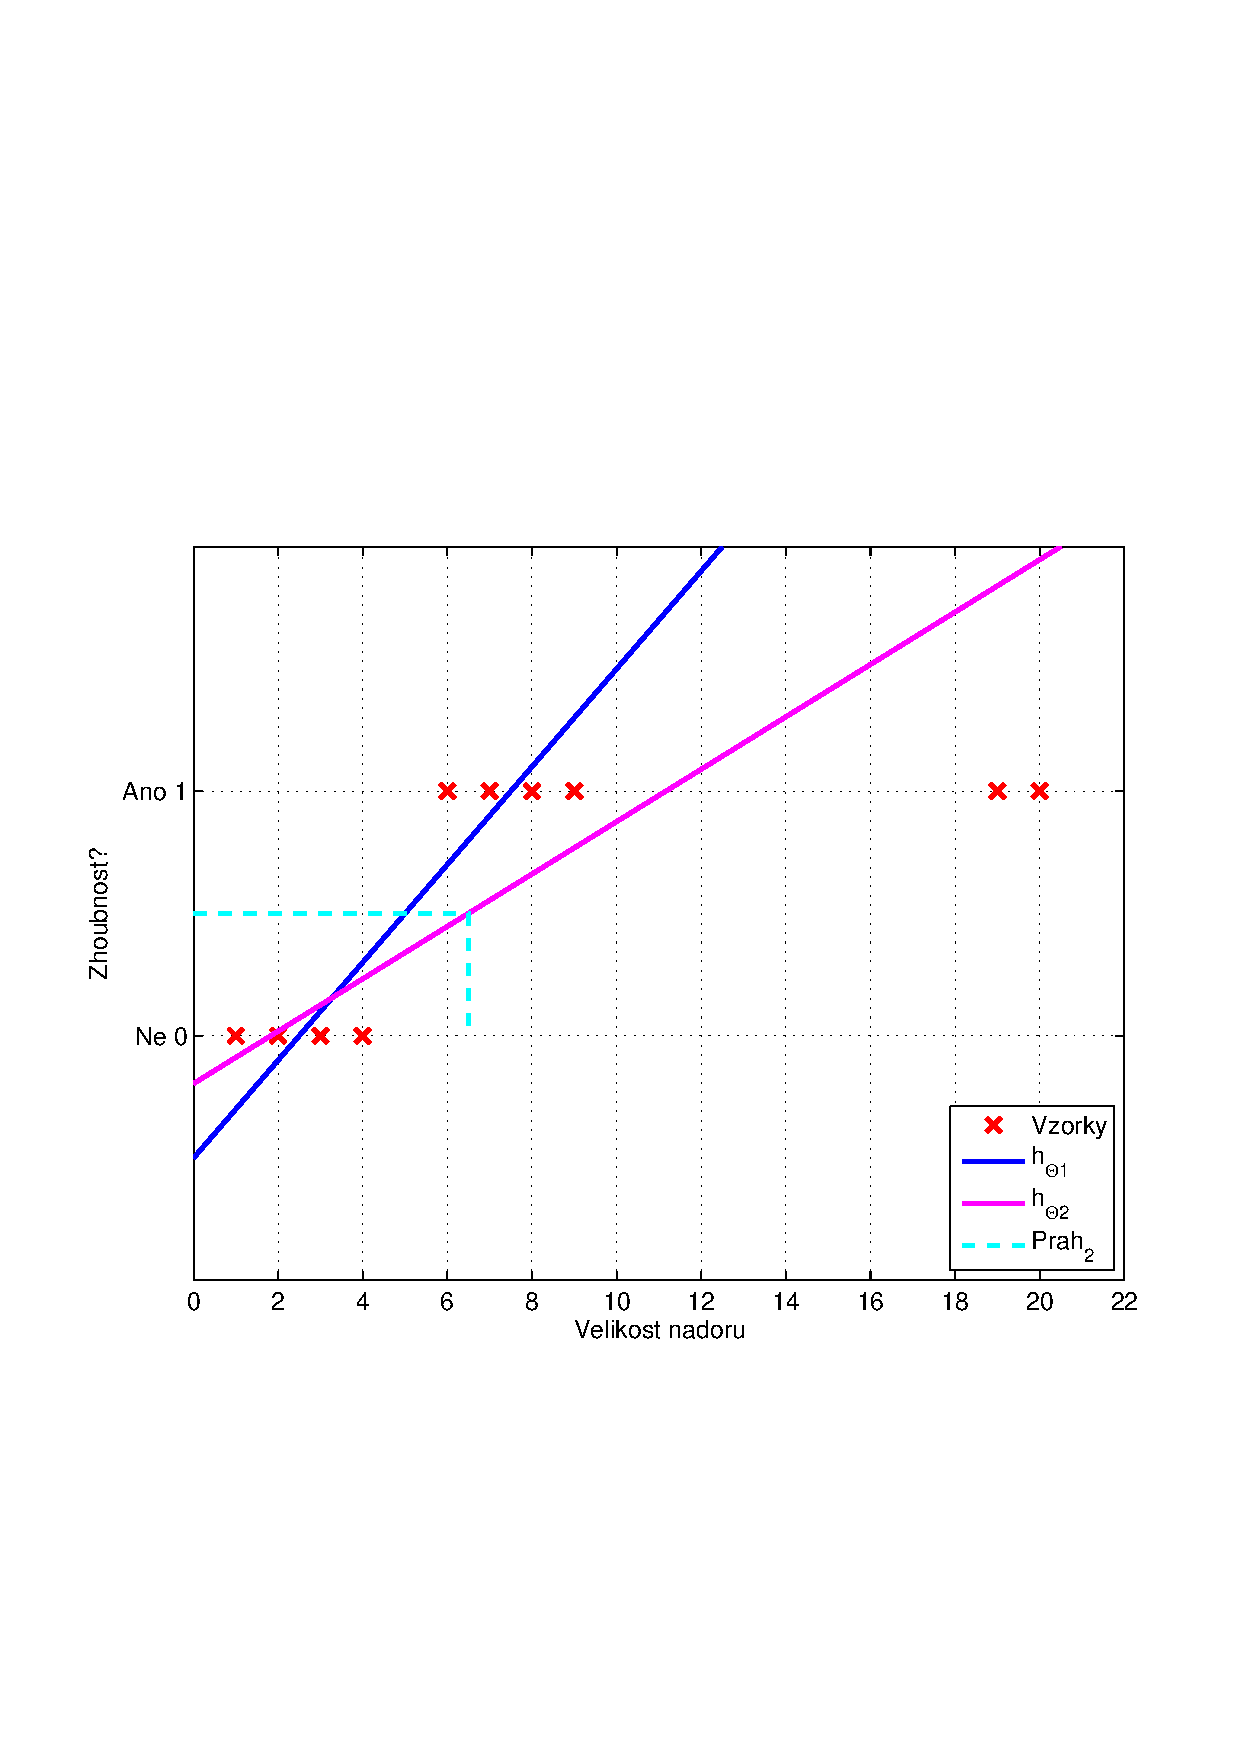
\includegraphics[width = \textwidth, trim = 2.5cm 7cm 2cm 9cm]{./Img/BinarniRegrese/prikladNadory/tumor_5st_example.pdf}
		\caption{Lineární regrese - určení rozhodovacího prahu a zobrazení jeho selhání při predikci.}
		\label{fig:nadory5}
	\end{minipage}%
\end{figure}}

\par{V tomto příkladě, lépe řečeno protipříkladě jsme si ukázali, proč je nevhodné využívat lineární regresi jako klasifikační algoritmus. Ve většině případů nefunguje správně. Pro klasifikaci na základě lineární regrese můžeme získat výsledek hypotézy $h_{\bm{\Theta}} > 1$ nebo $h_{\bm{\Theta}} < 0$, přičemž výsledek binární klasifikace je pouze $y = 0$ nebo $y = 0$. Proto bude nutné v~dalších kapitolách přijít se sofistikovanějším postupem binární regrese (klasifikace), která splňuje podmínku $0 \leq h_{\bm{\Theta}} \leq 1$.}




\newpage













%-----REPREZENTACE-HYPOTEZY-------------------------------------------------------------
\section{Reprezentace hypotézy}
\label{sec:BinarniRegreseReprezentaceHypotezy}

\par{V této kapitole si ukážeme, jak správně reprezentovat hypotézu, tedy jakou funkci je vhodné použít v případě problému klasifikace.}

\par{V sekci \ref{sec:BinarniRegreseKlasifikace} jsme zjistili, že bychom si pro binární regresní model přáli, aby platilo
\begin{equation}
	0 \leq h_{\bm{\Theta}} \left( \bm{x} \right) \leq 1,
\end{equation}
tedy aby výstupní hodnota byla mezi 0 a 1 (včetně). Pro reprezentaci hypotézy lineární regrese platí
\begin{equation}
	h_{\bm{\Theta}} \left( \bm{x} \right) = \bm{\Theta}^{\top} \bm{x},
\end{equation}
tuto hypotézu upravíme na tvar
\begin{equation}
	h_{\bm{\Theta}} \left( \bm{x} \right) = g \left( \bm{\Theta}^{\top} \bm{x} \right),
	\label{eq:Ghypoteza}
\end{equation}
kde funkce $g$ je definována následovně
\begin{equation}
	g \left( \bm{z} \right) = \frac{1}{1 + e^{-\bm{z}}},
	\label{eq:funkceSigmoidy}
\end{equation}
tato funkce se nazývá sigmoid funkce (Sigmoid function) nebo logistická/binární funkce (Logistic function). Jméno logistická funkce je důvod, proč vznik termín logistická/binární regrese. Pokud spojíme rovnice \ref{eq:Ghypoteza} a \ref{eq:funkceSigmoidy} získáme tvar
\begin{equation}
	h_{\bm{\Theta}} \left( \bm{x} \right) =  \frac{1}{1 + e^{- \bm{\Theta}^{\top} \bm{x}}} 
\end{equation}
a průběh grafu funkce $g \left( \bm{z} \right)$ lze vidět na Obr. \ref{fig:sigmoidFunction}.
\begin{figure}[!ht]
	\centering
	%trim option's parameter order: left bottom right top
	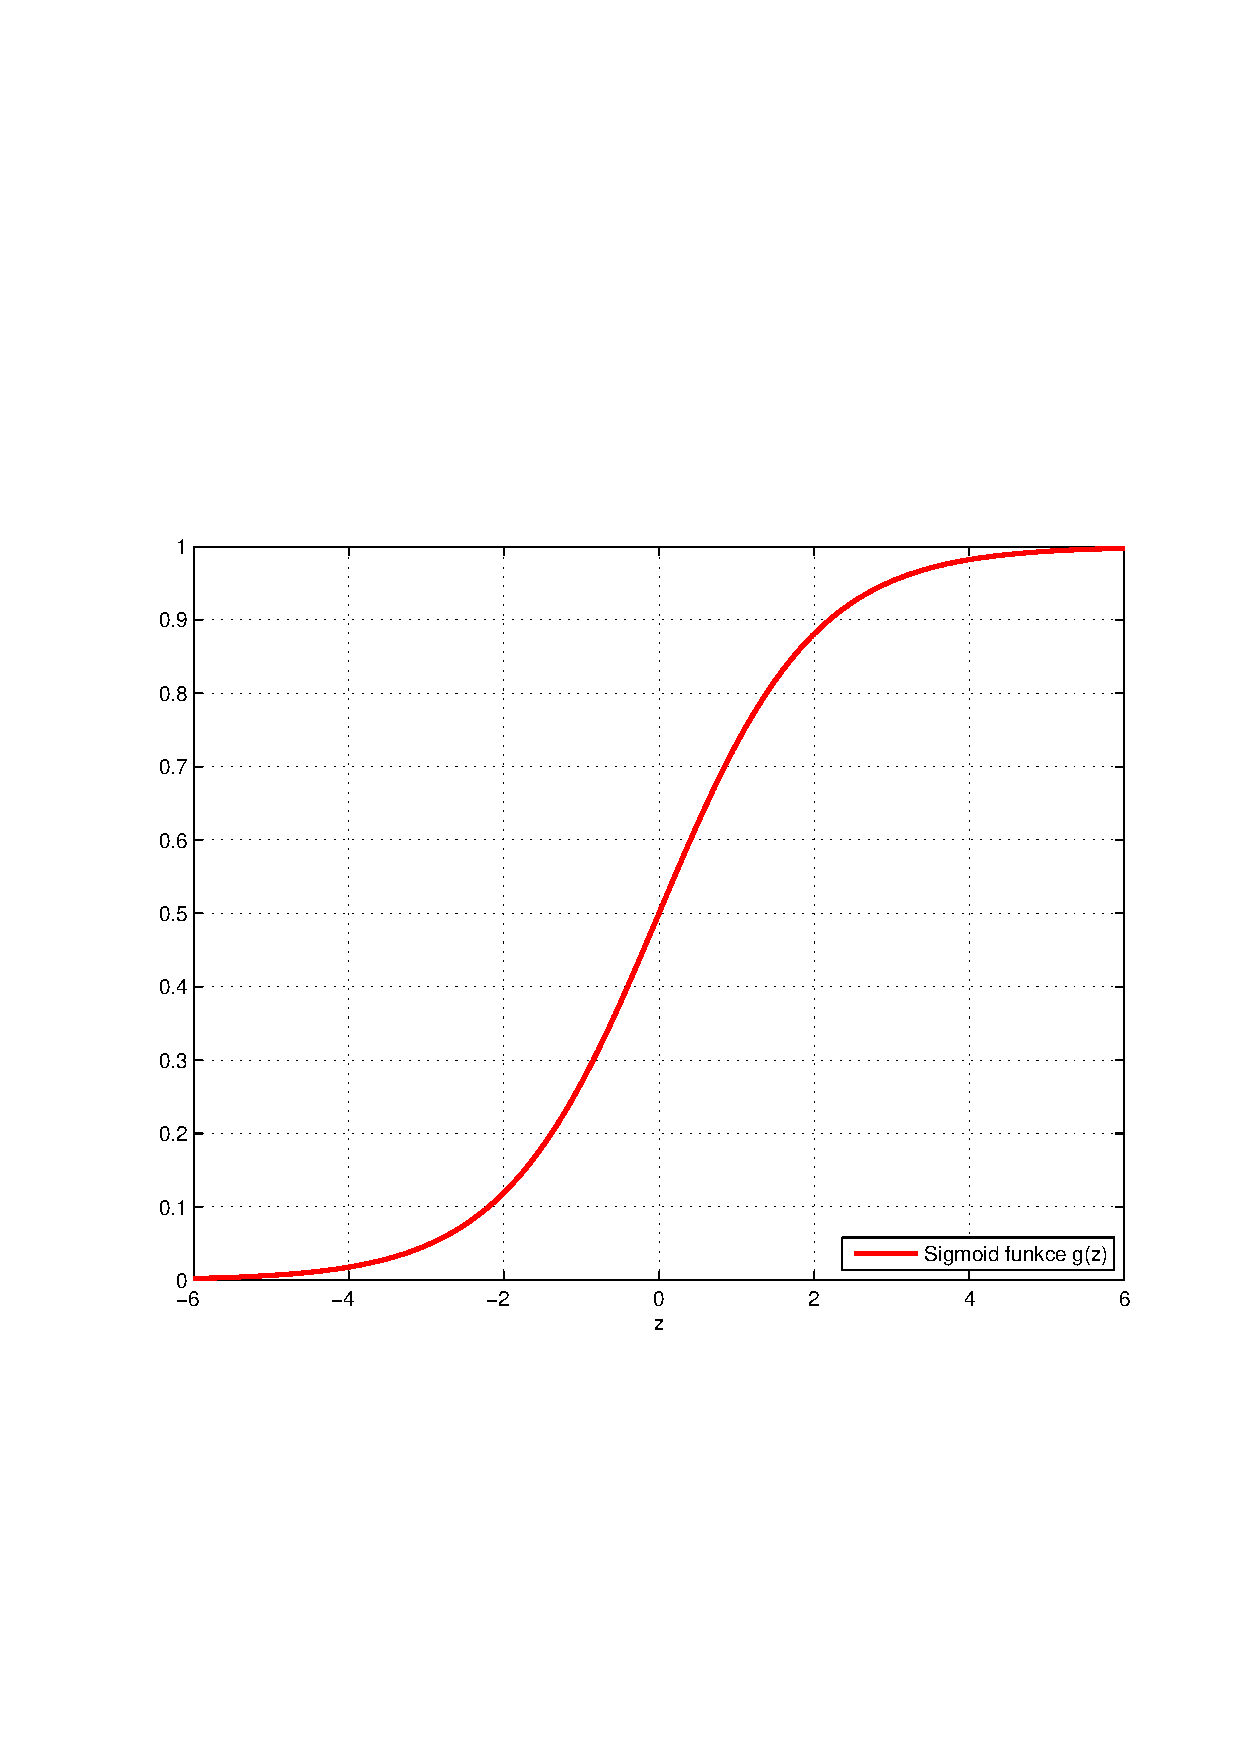
\includegraphics[width = 0.48\textwidth, trim = 2.5cm 7cm 2cm 9cm]{./Img/BinarniRegrese/sigmoidFunkce/sigmoidFunction.pdf}
	\caption{Sigmoidní funkce $g \left( z \right)$.}
	\label{fig:sigmoidFunction}
\end{figure}}
\par{Poznamenejme, že
\begin{eqnarray}
	\nonumber
	\lim_{z \to +\infty} &g \left( z \right) &= 1,\\
	\nonumber
	\lim_{z \to -\infty} &g \left( z \right) &= 0.
\end{eqnarray}}

\par{Nyní je potřeba, stejně jako dříve, přizpůsobit parametry $\bm{\Theta}$ našim datům, tedy pomocí trénovací množiny zvolit hodnoty parametrů $\bm{\Theta}$ a využít tyto parametry pro výpočet predikce.}

\par{Dále si povíme něco o interpretaci výstupu hypotézy. Hypotéza $h_{\bm{\Theta}} \left( \bm{x} \right) = $ odhadnutá pravděpodobnost, že výstup $y = 1$ na základě vstupních dat $\bm{x}$.}

\subsubsection*{Příklad}
\par{Pokud $\bm{x} = [ x_0,~x_1 ]^{\top} = [ 1,~$velikost nádoru$]^{\top}$ a $h_{\bm{\Theta}} \left( \bm{x} \right) = 0.7$, což říká pacientovi, že šance, že je nádor zhoubný je $70\%$. Nyní naše tvrzení zapíšeme formálněji
\begin{equation}
	h_{\bm{\Theta}} \left( \bm{x} \right) = P \left( y = 1 | \bm{x} ; \bm{\Theta} \right),
\end{equation}
neboli, pravděpodobnost, že $y = 1$, \uv{na základě dat $\bm{x}$}, parametrizovaná parametry $\bm{\Theta}$. V případě klasifikace víme, že výstup $y$ může nabývat pouze hodnot 0 nebo 1, proto platí
\begin{equation}
	P \left( y = 0 | \bm{x} ; \bm{\Theta} \right) + P \left( y = 1 | \bm{x} ; \bm{\Theta} \right) = 1,
\end{equation}
neboli
\begin{equation}
	P \left( y = 0 | \bm{x} ; \bm{\Theta} \right) = 1 - P \left( y = 1 | \bm{x} ; \bm{\Theta} \right).
\end{equation}}

\subsubsection*{Poznámka}
\par{Pravděpodobnost může nabývat hodnot $0-1$, neboli $0-100\%$.}





\newpage












%----------ROZHODOVACI-HRANICE-------------------------------------------------------------
\section{Rozhodovací hranice}
\label{sec:BinarniRegreseRozhodovaciHranice}

\par{V~této kapitole si povíme něco o~rozhodovací hranici, abychom získali větší ponětí o~výpočtu hypotézy binární regrese (klasifikace).}

\par{V kapitole \ref{sec:BinarniRegreseReprezentaceHypotezy} jsme si ukázali tvar hypotézy (sigmoid funkce)
\begin{equation}
	h_{\bm{\Theta}} \left( \bm{x} \right) = g \left( \bm{\Theta}^{\top} \bm{x} \right),
\end{equation}
kde
\begin{equation}
	g \left( \bm{z} \right) = \frac{1}{1 + e^{-\bm{z}}}
\end{equation}
a graf lze vidět na Obr. \ref{fig:sigmoidFunction2}.
\begin{figure}[!ht]
	\centering
	%trim option's parameter order: left bottom right top
	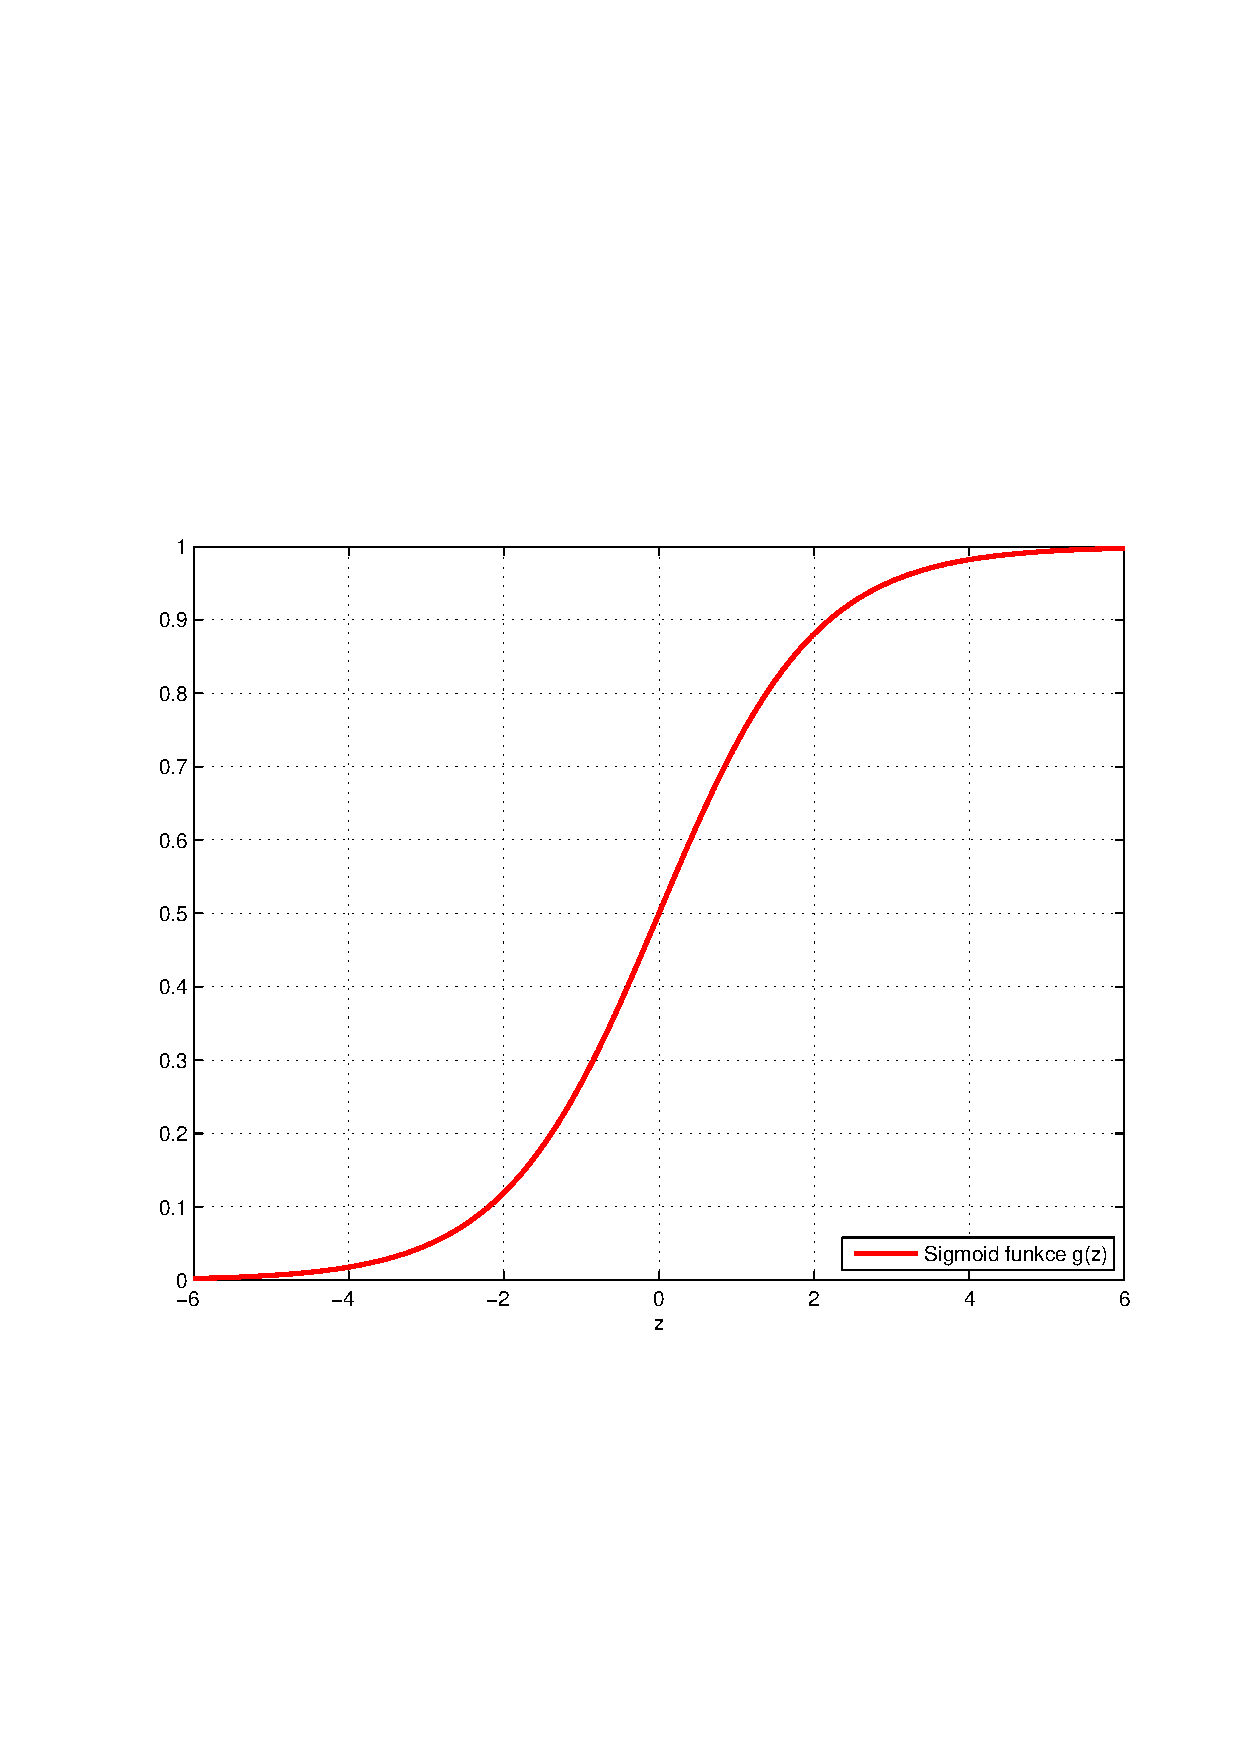
\includegraphics[width = 0.48\textwidth, trim = 2.5cm 7cm 2cm 9cm]{./Img/BinarniRegrese/sigmoidFunkce/sigmoidFunction.pdf}
	\caption{Sigmoidní funkce $g \left( z \right)$.}
	\label{fig:sigmoidFunction2}
\end{figure}}

\par{Podrobněji vysvětlíme, kdy naše hypotéza bude predikovat na výstupu 0 nebo 1. Konkrétně naše hypotéza bude na výstupu predikovat $y = 1$ v případě
\begin{equation}
	h_{\bm{\Theta}} \left( \bm{x} \right) = g \left( \bm{\Theta}^{\top} \bm{x} \right) = P \left( y = 1 | \bm{x}; \bm{\Theta} \right).
\end{equation}
Předpokládejme, že klasifikátor predikuje výstup $y = 1$ pokud $h_{\bm{\Theta}} \left( \bm{x} \right) \geq 0.5$, což platí pro $\bm{\Theta}^{\top} \bm{x} \geq 0$ a~klasifikátor predikuje výstup $y = 0$ pokud $h_{\bm{\Theta}} \left( \bm{x} \right) < 0.5$, což platí pro $\bm{\Theta}^{\top} \bm{x} < 0$.}

\newpage

\subsubsection*{Příklad - lineárně separabilní třídy}
\par{Předpokládejme, že máme trénovací sadu, která je znázorněna na Obr.~\ref{fig:decisionBoundary1} a~naše hypotéza má tvar
\begin{equation}
	h_{\bm{\Theta}} \left( \bm{x} \right) = g \left( \vartheta_0 + \vartheta_1 x_1 + \vartheta_2 x_2 \right).
	\label{eq:linearniHypotezaRovnice}
\end{equation}
Nyní se nebudeme zabývat tím, jak přizpůsobit parametry tomuto modelu. Předpokládejme, že $\bm{\Theta} = \left[ \vartheta_0,~\vartheta_1,~\vartheta2 \right]^{\top} = \left[ -3,~1,~1 \right]^{\top}$.}
\begin{figure}[!ht]
	\centering
	\begin{minipage}[b]{0.48\textwidth}
		%trim option's parameter order: left bottom right top
		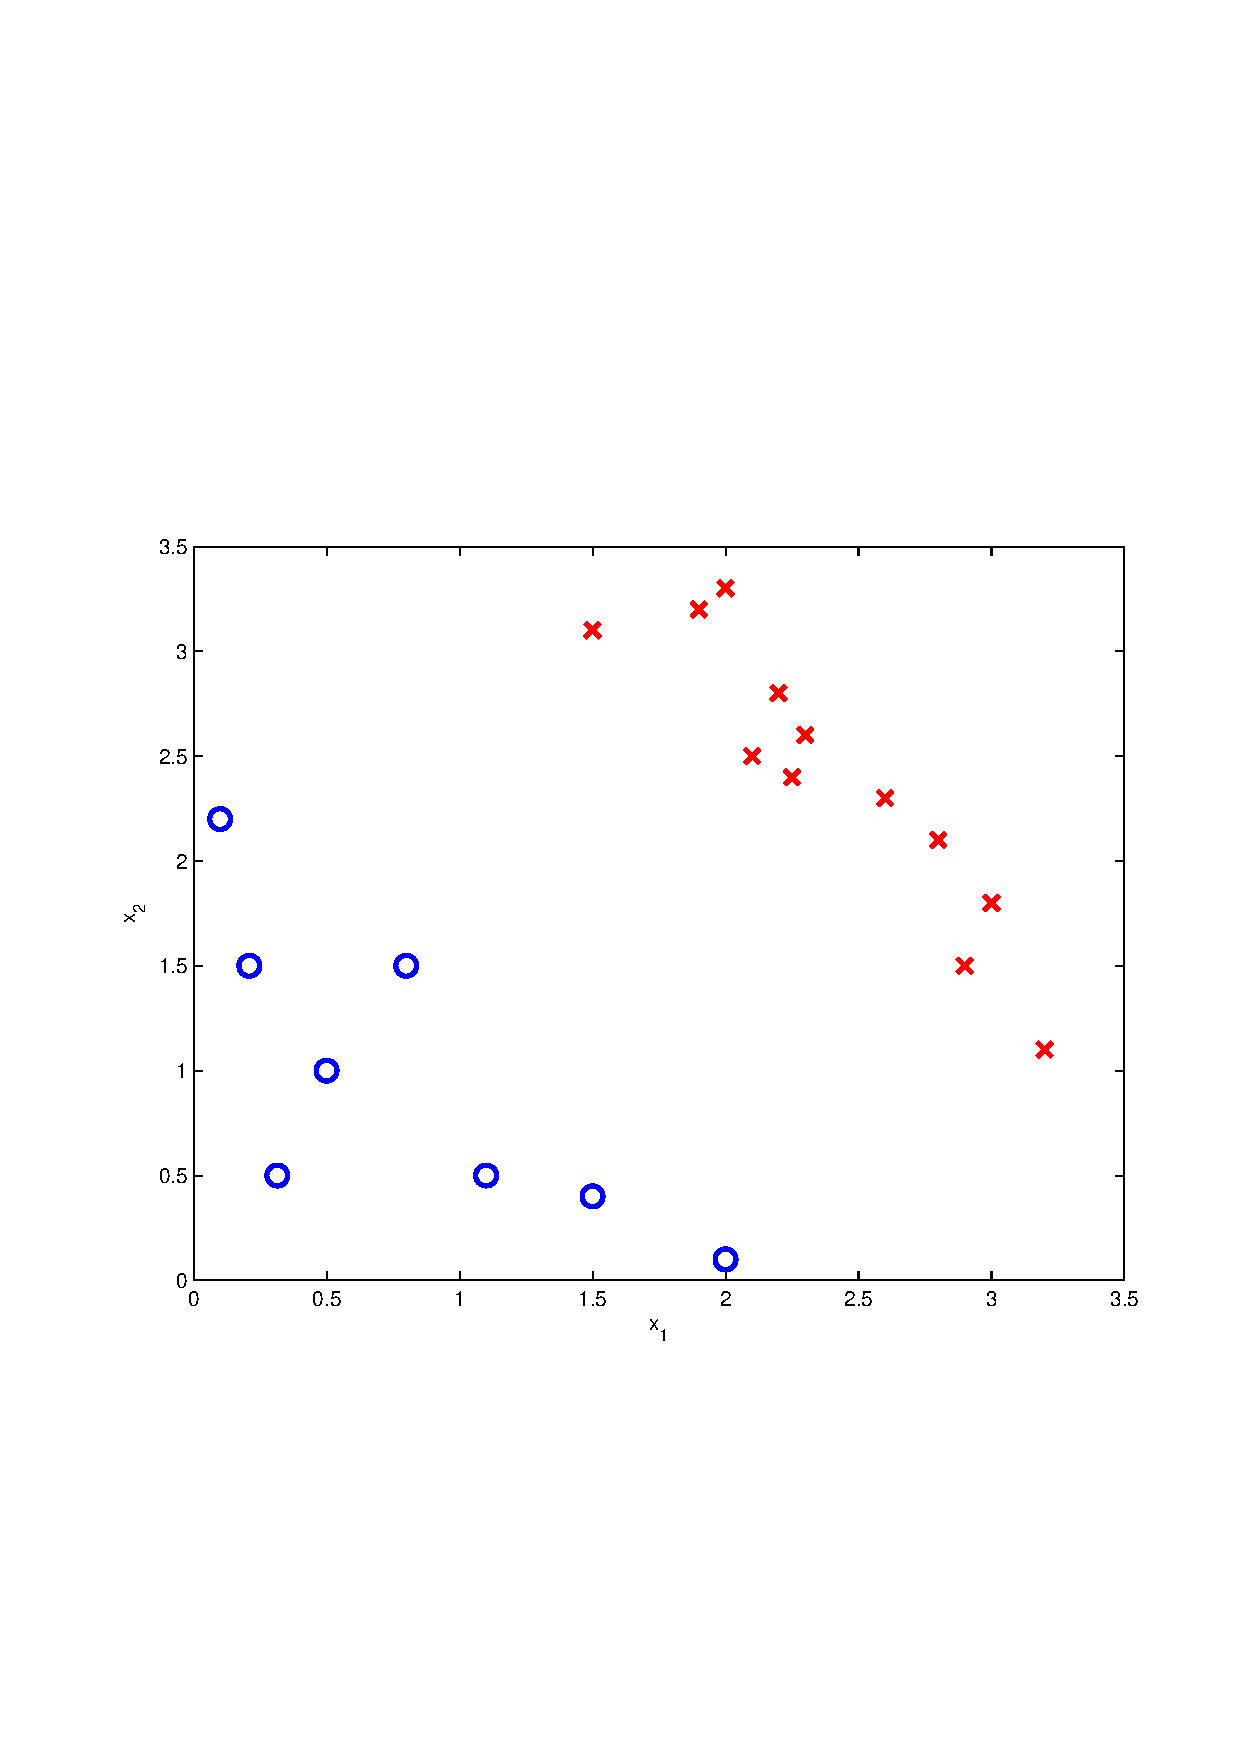
\includegraphics[width = \textwidth, trim = 2.5cm 7cm 2cm 9cm]{./Img/BinarniRegrese/decisionBoundary/decisionBoundary1.pdf}
		\caption{Vizualizace dvou tříd. \\ ~}
		\label{fig:decisionBoundary1}
	\end{minipage}%
	\hfill
	\begin{minipage}[b]{0.48\textwidth}
		%trim option's parameter order: left bottom right top
		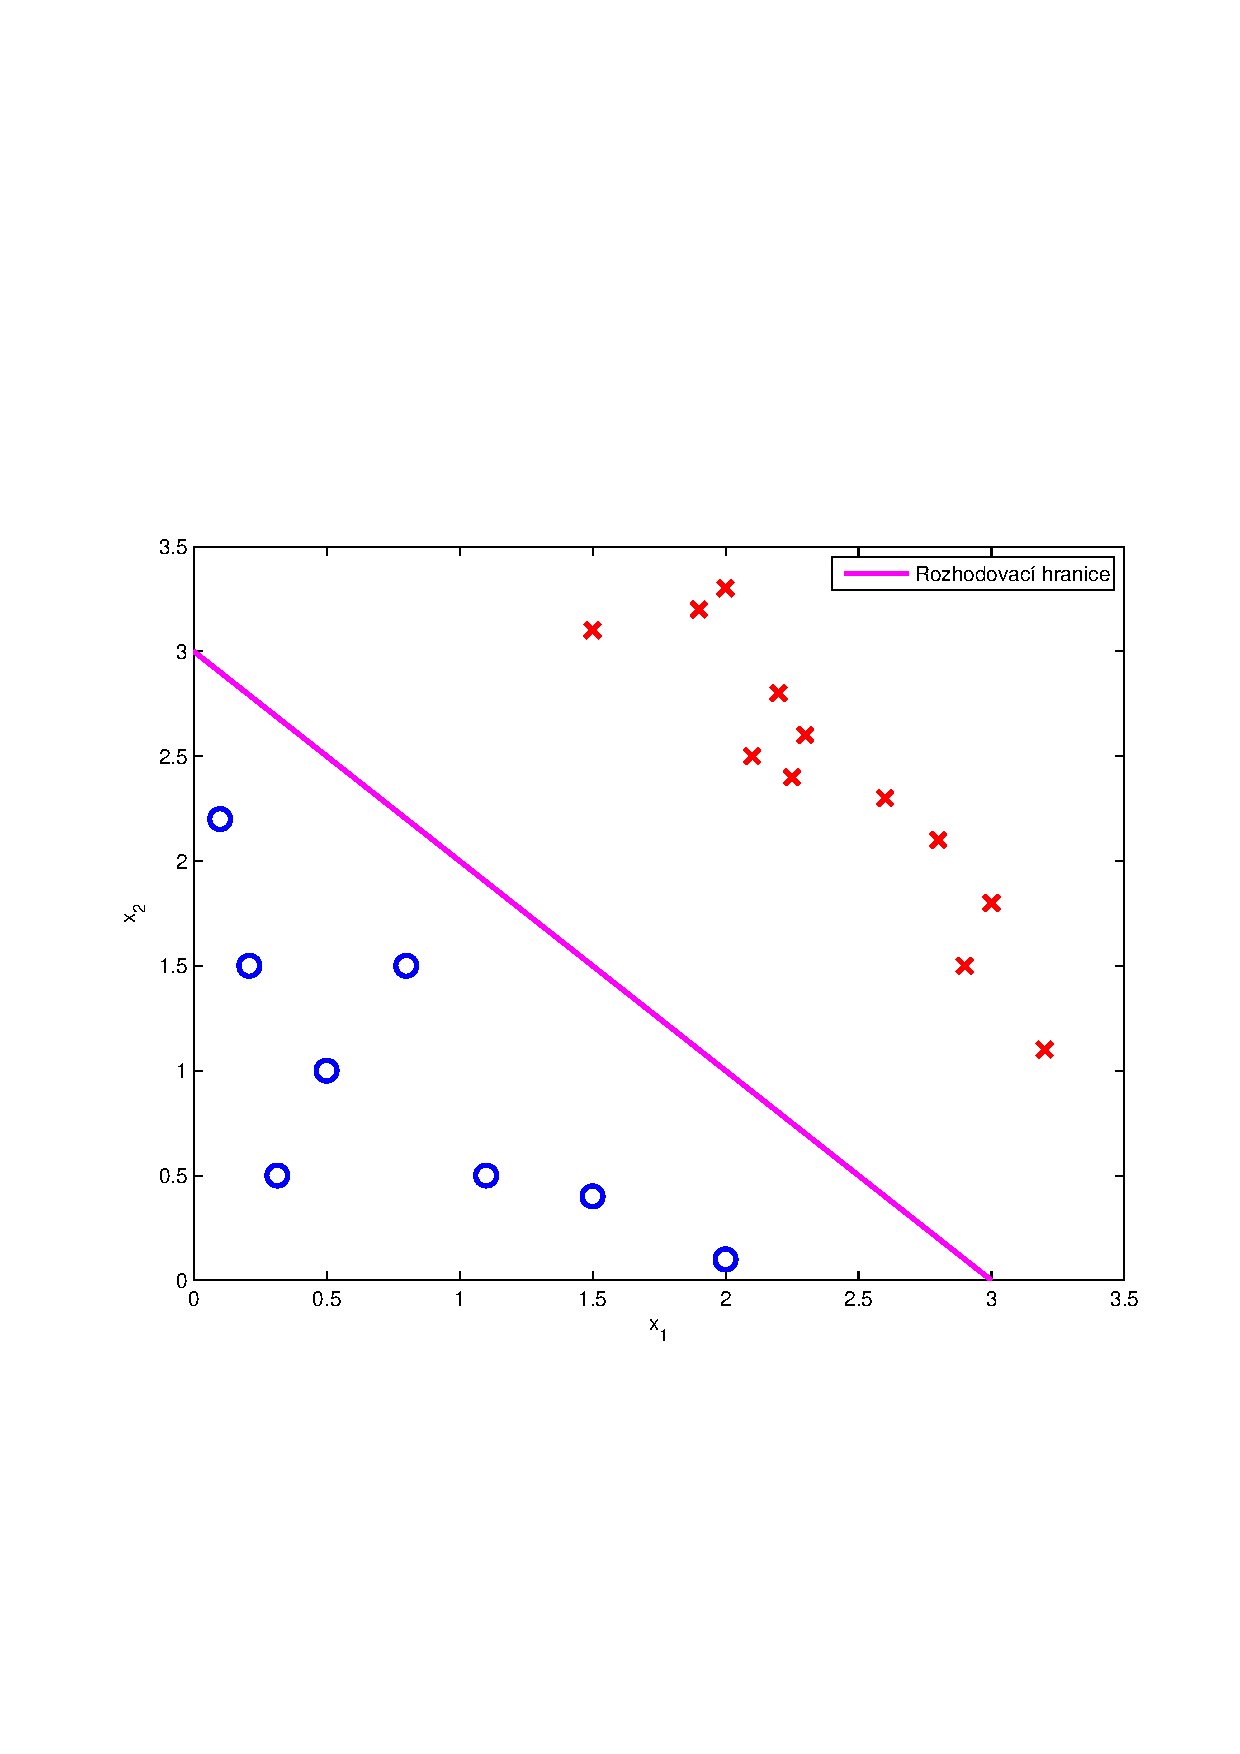
\includegraphics[width = \textwidth, trim = 2.5cm 7cm 2cm 9cm]{./Img/BinarniRegrese/decisionBoundary/decisionBoundary2.pdf}
		\caption{Vizualizace rozhodovací hranice.}
		\label{fig:decisionBoundary2}
	\end{minipage}%
\end{figure}

\par{Na příkladu si ukážeme, kdy hypotéza bude predikovat, jako výstup 0 a kdy 1. Hypotéza bude predikovat výstupní hodnotu $y = 1$ pokud
\begin{equation}
	-3 + x_1 + x_2 \geq 0
	\label{eq:prikladDecisionBoundary}
\end{equation}
($\bm{\Theta}^{\top} \bm{x} \geq 0$), jinými slovy pro všechna $x_1$ a $x_2$, které splňují rovnici \ref{eq:prikladDecisionBoundary} bude naše hypotéza predikovat výstup $y = 1$. Řešení rovnice \ref{eq:prikladDecisionBoundary} je naznačeno na Obr. \ref{fig:decisionBoundary2} a~odpovídají mu červené křížky nad rozhodovací hranicí.}

\par{V~případě, kdy $x_1 + x_2 = 3$, tak to odpovídá přesně $h_{\bm{\Theta}} \left( \bm{x} \right) = 0.5$. Jinak řečeno řešení odpovídá přesně rozhodovací hranici mezi třídami.}

\newpage

\subsubsection*{Příklad - lineárně neseparabilní třídy}
\par{Předpokládejme složitější příklad, kde nelze jednoduše použít binární regresi (lineární rozhodovací hranici) a~musíme využít polynomiální regrese, tedy musíme využít vyšší stupně polynomů jako příznaky viz Obr. \ref{fig:decisionBoundary3}.}
\begin{figure}[!ht]
	\centering
	\begin{minipage}[t]{0.48\textwidth}
		%trim option's parameter order: left bottom right top
		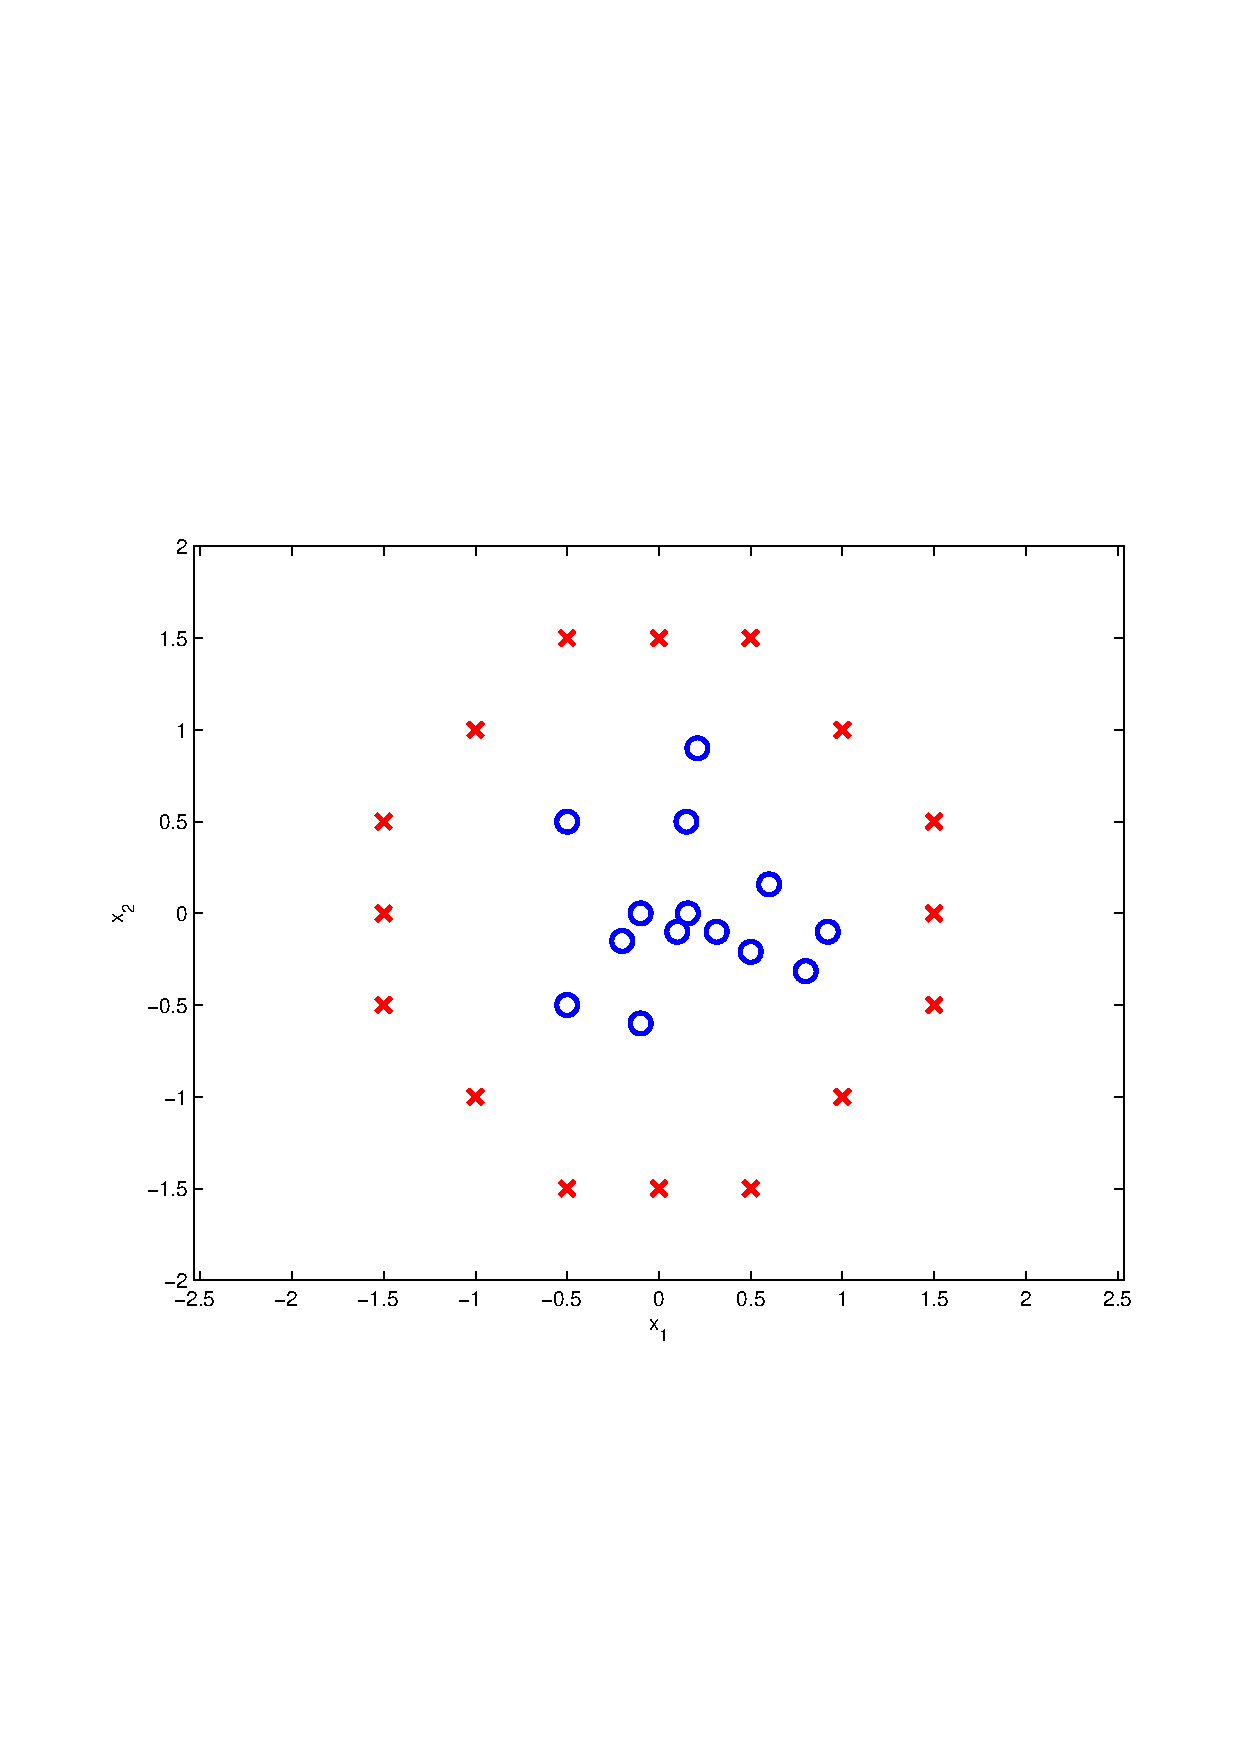
\includegraphics[width = \textwidth, trim = 2.5cm 7cm 2cm 9cm]{./Img/BinarniRegrese/decisionBoundary/decisionBoundary3.pdf}
		\caption{Vizualizace lineárně neseparabilních tříd.}
		\label{fig:decisionBoundary3}
	\end{minipage}%
	\hfill
	\begin{minipage}[t]{0.48\textwidth}
		%trim option's parameter order: left bottom right top
		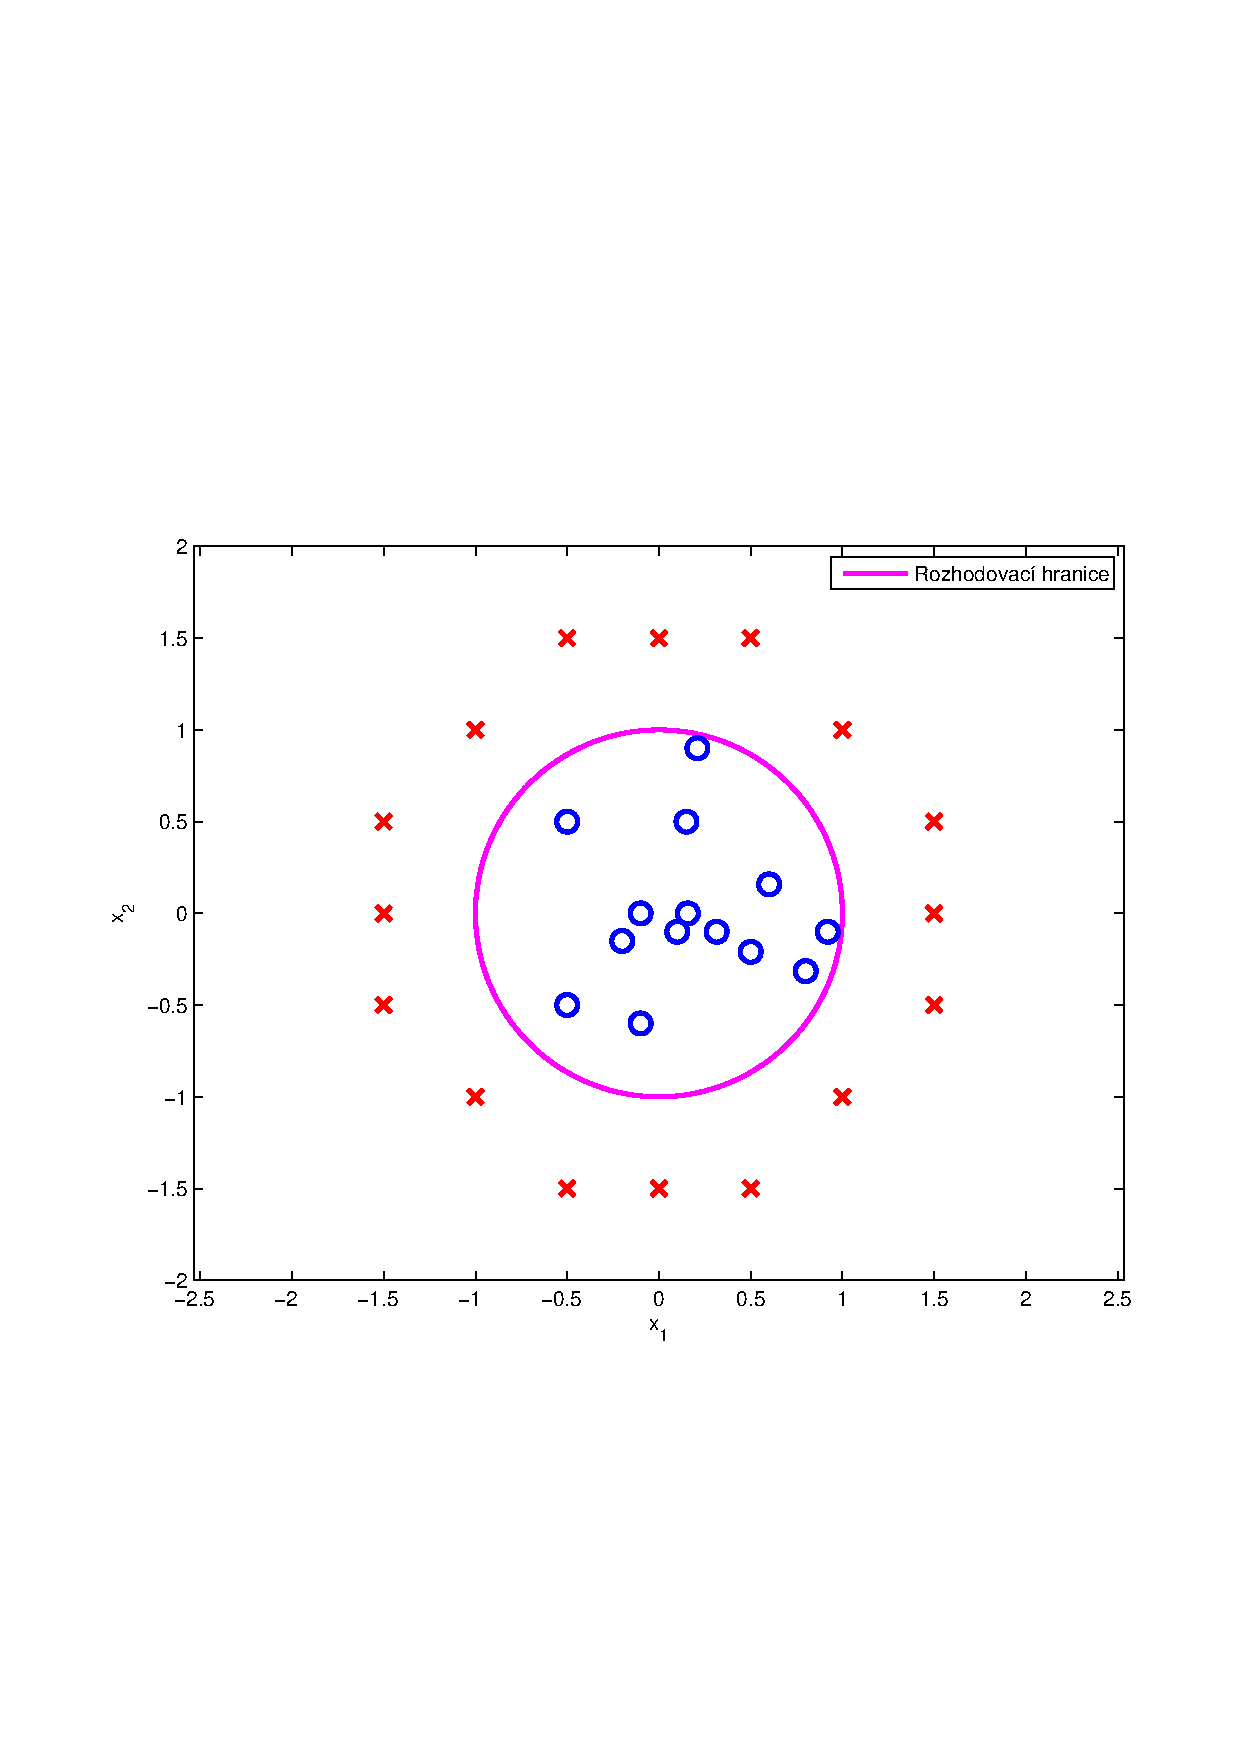
\includegraphics[width = \textwidth, trim = 2.5cm 7cm 2cm 9cm]{./Img/BinarniRegrese/decisionBoundary/decisionBoundary4.pdf}
		\caption{Vizualizace lineárně neseparabilních tříd společně s~rozhodovací hranicí.}
		\label{fig:decisionBoundary4}
	\end{minipage}%
\end{figure}

\par{Naše hypotéza má tvar $h_{\bm{\Theta}} \left( \bm{x} \right) = g \left( \vartheta_0 + \vartheta_1 x_1 + \vartheta_2 x_2 + \vartheta_3 x_1^2 + \vartheta_4 x_2^2 \right)$, kde jsme oproti předcházejícímu příkladu (rovnice \ref{eq:linearniHypotezaRovnice}) přidali dva příznaky $x_1^2$ a $x_2^2$ a~máme 5~parametrů $\vartheta_{0,\ldots,4}$. Nebudeme zabývat tím, jak vypočítat parametry $\bm{\Theta}$ (bude popsáno v~následujících sekcích), řekněme, že $\bm{\Theta} = \left[ \vartheta_0,~\vartheta_1,~\vartheta_2,~\vartheta_3,~\vartheta_4 \right]^{\top} = \left[ -1,~0,~0,~1,~1 \right]^{\top}$. Což znamená, že naše hypotéza bude predikovat výstup $y = 1$ pokud $-1 + x_1^2 + x_2^2 \geq 0$ (pro směr ven od rozhodovací hranice), tato rovnice odpovídá rovnici kružnice $x_1^2 + x_2^2 = 1$ o~poloměru $r = 1$. Rozhodovací hranice je vidět na Obr.~\ref{fig:decisionBoundary4}.}

\subsubsection*{Poznámka}
\par{Rozhodovací hranice je vlastnost hypotézy, konkrétně parametrů $\bm{\Theta}$, není to vlastnost trénovací sady. Trénovací sada je pouze využita k nalezení parametrů hypotézy~$\bm{\Theta}$.}





\newpage















%----------------------------------------------------------------------------------------
\section{Ztrátová funkce}
\label{sec:BinarniRegreseZtratovaFunkce}

\par{V této sekci si povíme jak vypočítat parametry $\bm{\Theta}$ pro binární regresi / klasifikaci.}

\par{Definujme problém učení s učitelem pro binární regresní model. Mějme trénovací množinu
\begin{equation}
	\{ \left( \bm{x}^{\left( 1 \right)}, y^{\left( 1 \right)} \right), \left( \bm{x}^{\left( 2 \right)}, y^{\left( 2 \right)} \right), \ldots , \left( \bm{x}^{\left( m \right)}, y^{\left( m \right)} \right) \}
\end{equation}
o velikosti $m$ vzorků, kde
\begin{equation}
	\bm{x}^{\left( i \right)} = \left[ x_0,~x_1,~\ldots,~x_n \right]^{\top},
\end{equation}
$\bm{x}^{\left( i \right)} \in \mathrm{R}^{n+1}$ a $x_0 = 1$, $y \in \{ 0,1 \}$. Naše hypotéza má tvar
\begin{equation}
	h_{\bm{\Theta}} \left( \bm{x} \right) = \frac{1}{1 + e^{-\bm{\Theta}^{\top} \bm{x}}}.
\end{equation}}

\par{Nyní si položme zásadní otázku, jak zvolit parametry $\bm{\Theta}$ v závislosti na naší trénovací množině?}

\par{Připomeňme si ztrátovou funkci $J \left( \bm{\Theta} \right)$ pro lineární regresi (viz sekce \ref{sec:LinearniRegreseZtratovaFunkce}), kterou zapíšeme v následujícím tvaru
\begin{equation}
	J \left( \bm{\Theta} \right) = \frac{1}{m} \sum_{i=1}^{m} \frac{1}{2} \left( h_{\Theta} \left( \bm{x}^{\left( i \right)} \right) - y^{\left( i \right)} \right)^2,
\end{equation}
dále můžeme ztrátovou funkci přepsat do tvaru
\begin{equation}
	J \left( \bm{\Theta} \right) = \frac{1}{m} \sum_{i=1}^{m} Cena \left( h_{\bm{\Theta}} \left( \bm{x}^{\left( i \right)} \right), y^{\left( i \right)} \right),
	\label{eq:JcenaX}
\end{equation}
kde
\begin{equation}
	Cena \left( h_{\bm{\Theta}} \left( \bm{x}^{\left( i \right)} \right), y^{\left( i \right)} \right) = \frac{1}{2} \left( h_{\bm{\Theta}} \left( \bm{x}^{\left( i \right)} \right) - y^{\left( i \right)} \right)^2.
	\label{eq:cenaX}	
\end{equation}
Nyní lze z rovnice \ref{eq:JcenaX} lépe vidět, že ztrátová funkce je $\frac{1}{m}$ krát součet $Cen$ přes trénovací sadu. Rovnici \ref{eq:cenaX} lze dále zjednodušit vynecháním horních indexů
\begin{equation}
	Cena \left( h_{\bm{\Theta}} \left( \bm{x} \right), y \right) = \frac{1}{2} \left( h_{\Theta} \left( \bm{x} \right) - y \right)^2
\end{equation}
a říká nám jakou $Cenu$ zaplatíme pokud výstupní hodnota hypotézy bude $h_{\bm{\Theta}} \left( \bm{x} \right)$ a výstupní informace od učitele bude hodnota $y$.}

\par{Tento předpis \ref{eq:cenaX} pro výpočet $Ceny$ platí pro lineární regresi. Avšak v této sekci se zajímáme o binární regresi. Pokud bychom chtěli minimalizovat tuto ztrátovou funkci v rovnici \ref{eq:JcenaX}, tak tato funkce může být nekonvexní vzhledem k parametrům $\bm{\Theta}$ (není zaručeno, že dosáhneme globálního minima, jako v případě konvexní ztrátové funkce).}

\par{Uveďme si ztrátovou funkci, která se využívá při binární regresi
\begin{equation}
	\label{eq:ztratovaFunkceBinarniRegrese}
	Cena \left( h_{\bm{\Theta}} \left( \bm{x} \right), y \right) = \left\{
	\begin{array}{r}
		{- \log \left( h_{\bm{\Theta}} \left( \bm{x} \right) \right), \quad \textrm{pro}~y = 1} \\
		{- \log \left( 1 - h_{\bm{\Theta}} \left( \bm{x} \right) \right), \quad \textrm{pro}~y = 0}
	\end{array}
	\right.
\end{equation}
jinými slovy lze říci, že se jedná jakou ztrátu (kolik nás stojí) utrpíme pokud $y = 0$ nebo $y = 1$.}


\newpage

\par{Nyní si ztrátovou funkci pro binární regresi, z rovnice \ref{eq:ztratovaFunkceBinarniRegrese}, rozebereme podrobněji. Na Obr. \ref{fig:ztratovaFunkce3} lze vidět průběh ztrátové funkce.
\begin{figure}[!ht]
	\centering
	%trim option's parameter order: left bottom right top
	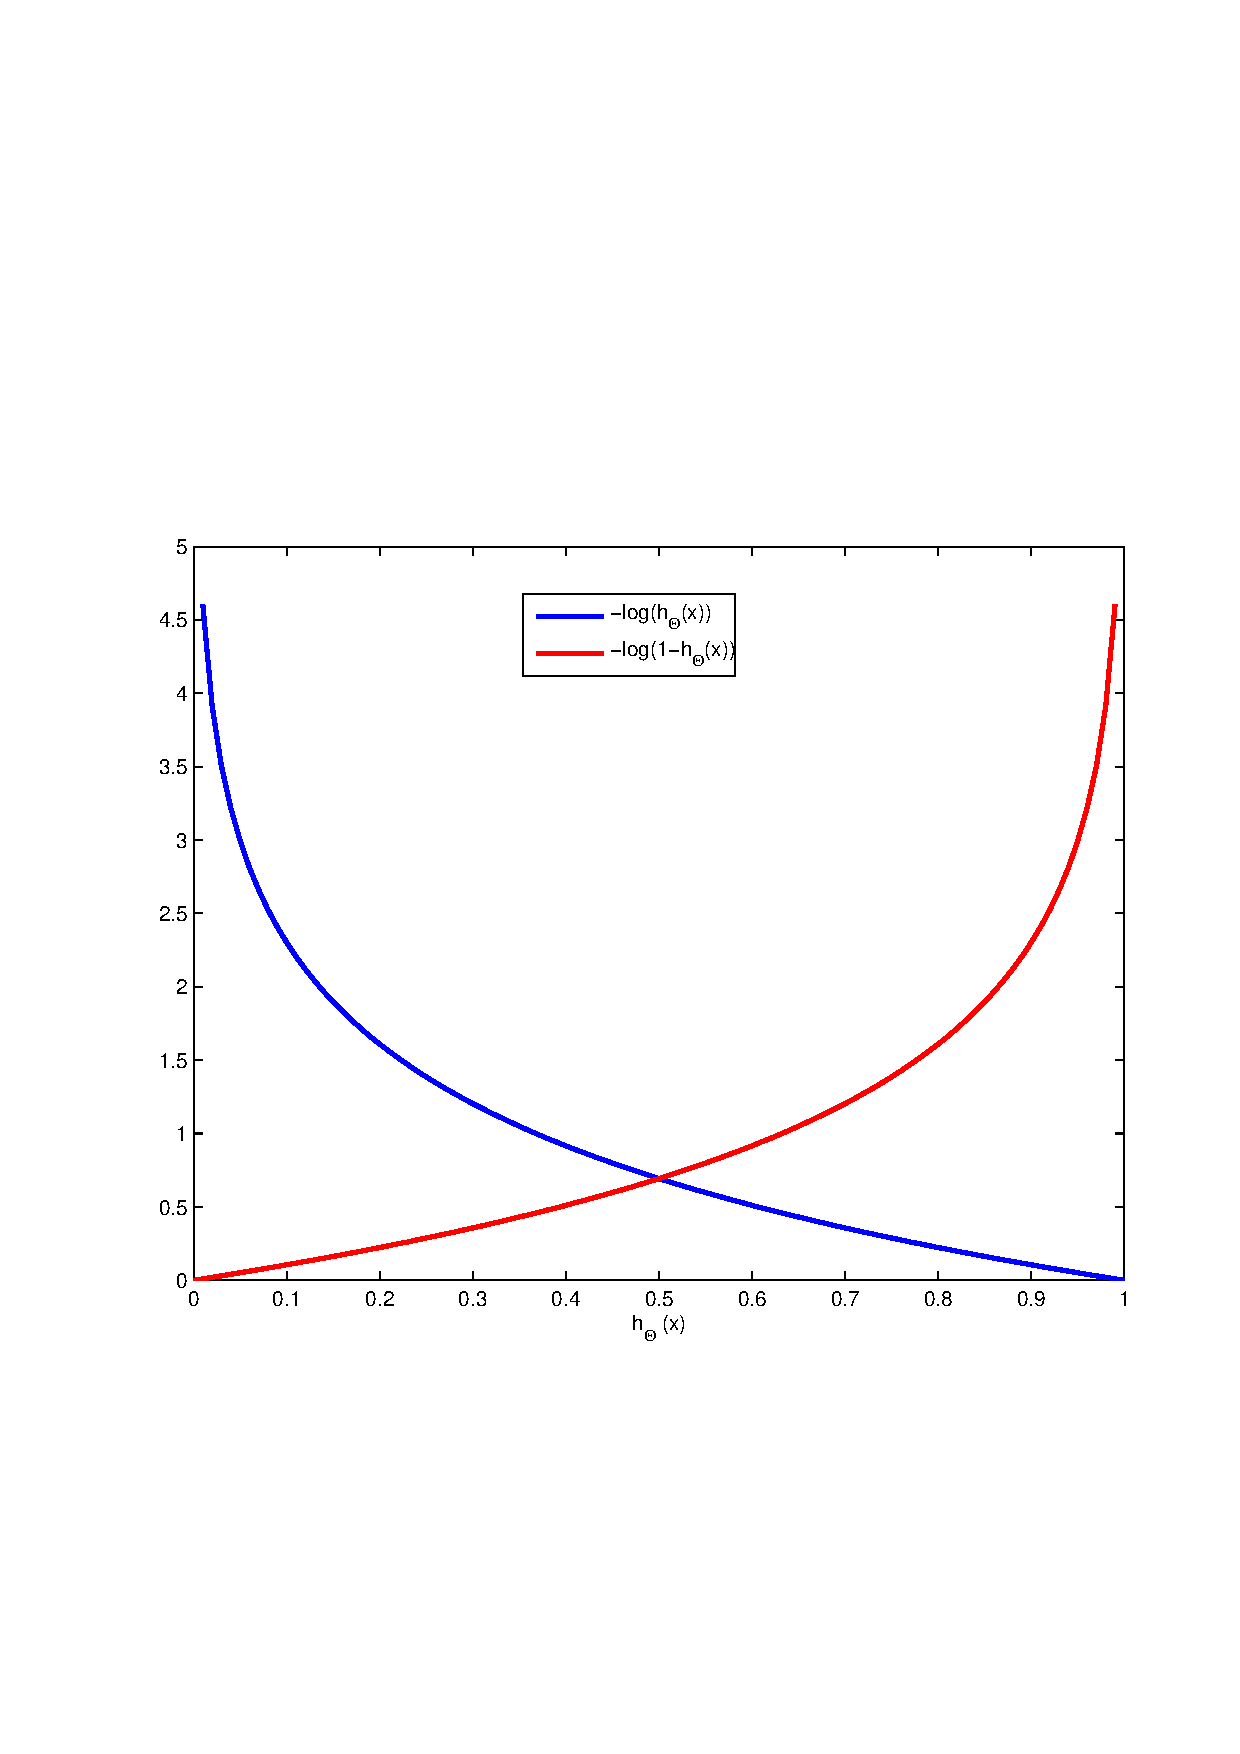
\includegraphics[width = 0.48\textwidth, trim = 2.5cm 7cm 2cm 9cm]{./Img/BinarniRegrese/ztratovaFunkce/ztratovaFunkce3.pdf}
	\caption{Průběh ztrátové funkce.}
	\label{fig:ztratovaFunkce3}
\end{figure}}

\par{Pokud bude $y = 1$ a naše hypotéza $h_{\bm{\Theta}} \left( \bm{x} \right) = 1$, tak utrpíme ztrátu rovnu $Cena = 0$. Ale pokud se bude hodnota hypotézy zmenšovat $h_{\bm{\Theta}} \left( \bm{x} \right) \rightarrow 0$, tak se utrpěná ztráta bude zvětšovat $Cena \rightarrow \infty$. V druhém případě pokud $h_{\bm{\Theta}} \left( \bm{x} \right) = 0$ (predikce $P \left( y = 1 | \bm{x}; \bm{\Theta} \right) = 0$), ale $y = 1$, tak utrpěná ztráta bude velmi velká.}

\par{Pro $y = 0$ platí obdobně druhá část rovnice \ref{eq:ztratovaFunkceBinarniRegrese}.}




\newpage
















%----------------------------------------------------------------------------------------
\section{Zjednodušená ztrátová funkce a gradientní metoda}

\par{Naše ztrátová funkce $J \left( \bm{\Theta} \right)$ ve tvaru
\begin{equation}
	J \left( \bm{\Theta} \right) = \frac{1}{m} \sum_{i=1}^{m} Cena \left( h_{\bm{\Theta}} \left( \bm{x}^{\left( i \right)} \right), y^{\left( i \right)} \right),
	\label{eq:JcenaXpodruhe}
\end{equation}
kde
\begin{equation}
	\label{eq:ztratovaFunkceBinarniRegrese2}
	Cena \left( h_{\bm{\Theta}} \left( \bm{x} \right), y \right) = \left\{
	\begin{array}{r}
		{- \log \left( h_{\bm{\Theta}} \left( \bm{x} \right) \right), \quad \textrm{pro}~y = 1} \\
		{- \log \left( 1 - h_{\bm{\Theta}} \left( \bm{x} \right) \right), \quad \textrm{pro}~y = 0}
	\end{array}
	\right.
\end{equation}
poznamenejme že $y = 0$ nebo $y = 1$ (pokaždé, žádná jiná možnost není).}

\par{Naší $Cenu$ z rovnice \ref{eq:ztratovaFunkceBinarniRegrese2} můžeme zapsat v jedné rovnici, která má tvar
\begin{equation}
	Cena \left( h_{\bm{\Theta}} \left( \bm{x} \right), y \right) = - y \log \left( h_{\bm{\Theta}} \left( \bm{x} \right) \right) - \left( 1 - y \right) \log \left( 1 - h_{\bm{\Theta}} \left( \bm{x} \right) \right),
	\label{eq:cena1rovnice}
\end{equation}
pokud $y = 1$, tak rovnice \ref{eq:cena1rovnice} přechází na první část rovnice \ref{eq:ztratovaFunkceBinarniRegrese2} a pokud $y = 0$, tak rovnice \ref{eq:cena1rovnice} přechází na druhou část rovnice \ref{eq:ztratovaFunkceBinarniRegrese2}.}

\par{Po spojení a úpravě rovnic \ref{eq:cena1rovnice} a \ref{eq:JcenaXpodruhe} získáme výsledný tvar
\begin{equation}
		J \left( \bm{\Theta} \right) = - \frac{1}{m} \left[ \sum_{i=1}^{m} y^{\left( i \right)} \log \left( h_{\bm{\Theta}} \left( \bm{x}^{\left( i \right)} \right) \right) + \left( 1 - y^{\left( i \right)} \right) \log \left( 1 - h_{\bm{\Theta}} \left( \bm{x}^{\left( i \right)} \right) \right) \right].
		\label{eq:ztratovaFunkceJbinarniRegrese}
\end{equation}}

\par{Cílem je nalézt takové parametry $\bm{\Theta}$, které minimalizují ztrátovou funkci $J$
\begin{equation}
	\min_{\bm{\Theta}} J \left( \bm{\Theta} \right),
\end{equation}
a následně pro vypočítáme predikci naší hypotézy (na základě nového vstupu $x$) 
\begin{equation}
	h_{\bm{\Theta}} \left( \bm{x} \right) = \frac{1}{1 + e^{ - \bm{\Theta}^{\top} \bm{x}}}.
\end{equation}}

\par{Nyní můžeme konečně zapsat celý gradientní algoritmus, opakuj
\begin{equation}
	\vartheta_j = \vartheta_j - \alpha \frac{\partial}{\partial \vartheta_j} J \left( \bm{\Theta} \right),
	\label{eq:gradientDescentBinaryRegresionAlgorithm}
\end{equation}
po každé iteraci aktualizuj všechny parametry $\vartheta_j$ najednou dokud algoritmus nedokonverguje.}

\subsubsection*{Poznámka}
\par{V rovnici \ref{eq:gradientDescentBinaryRegresionAlgorithm} bude využit tvar
\begin{equation}
	\frac{\partial}{\partial \vartheta_j} J \left( \bm{\Theta} \right) = \frac{1}{m} \sum_{i = 1}^{m} \left( h_{\bm{\Theta}} \left( \bm{x}^{\left( i \right)} \right) - y^{\left( i \right)} \right) \bm{x}_j^{\left( i \right)}.
\end{equation} a proto je výhodnější psát rovnici \ref{eq:gradientDescentBinaryRegresionAlgorithm} ve tvaru
\begin{equation}
		\vartheta_j = \vartheta_j - \alpha \sum_{i = 1}^{m} \left( h_{\bm{\Theta}} \left( \bm{x}^{\left( i \right)} \right) - y^{\left( i \right)} \right) \bm{x}_j^{\left( i \right)}.
\end{equation}}

\par{Algoritmus vypadá totožně jako v případě lineární regrese (viz \ref{eq:NDgradientDescentVysledna}) s rozdílnou hypotézou $h_{\bm{\Theta}} \left( \bm{x} \right)$, v případě lineární regrese
\begin{equation}
	h_{\bm{\Theta}} \left( \bm{x} \right) = \bm{\Theta}^{\top} \bm{x}
\end{equation}
a v případě binární regrese se jedná o
\begin{equation}
	h_{\bm{\Theta}} \left( \bm{x} \right) = \frac{1}{1 + e^{- \bm{\Theta}^{\top} \bm{x}}}.
\end{equation}}

\subsubsection*{Poznámka}
\par{Při výpočtu parametrů $\bm{\Theta}$ pomocí gradientního algoritmu v případě binární regrese je také vhodné využít Features scaling, jako v případě lineární regrese (viz sekce \ref{sec:featuresScaling}).}



\newpage



















%----------------------------------------------------------------------------------------
\section{Pokročilé algoritmy optimalizace}

\par{V této sekci si uvedeme příklady několika pokročilejších algoritmů optimalizace, které jsou lépe využitelné pro velké problémy strojového učení, kde je například velký počet příznaků.}

\par{Připomeňme náš optimalizační problém, máme ztrátovou funkci $J \left( \bm{\Theta} \right)$ a chceme jí minimalizovat
\begin{equation}
	\min_{\bm{\Theta}} J \left( \bm{\Theta} \right).
\end{equation}
Musíme tedy znát rovnice pro výpočet $J \left( \bm{\Theta} \right)$ a $\frac{\partial}{\partial \vartheta_j} J \left( \bm{\Theta} \right)$ následně můžeme využít zmíněný gradientní algoritmus, nebo nějakou z pokročilejších optimalizačních metod jako jsou například
\begin{table}[!ht]
\begin{center}
\begin{tabular}{r|c|c}
	{Název algoritmu} & {Výhody} & {Nevýhody}\\
	\hline
	{Conjugate gradient} & {Nemusí se volit} & {Více složité}\\
	{BFGS} & {konstanta učení $\alpha$.} & {}\\
	{L-BFGS} & {Rychlejší než gradientní metoda.} & {}
\end{tabular}
	\caption{Příklady pokročilejších optimalizačních algoritmů.}
\end{center}
\end{table}}

\subsubsection*{Příklad}
\par{Nyní si uvedeme příklad společně s jeho implementací v~MATLABu. Mějme vektor parametrů $\bm{\Theta} = \left[ \vartheta_1,~\vartheta_2 \right]^{\top}$ a ztrátovou funkci $J \left( \bm{\Theta} \right) = \left( \vartheta_1 - 5 \right)^2 + \left( \vartheta_2 - 5 \right)^2,$ dále vypočteme parciální derivace ztrátové funkce
\begin{eqnarray}
	\label{eq:prGrad1}
	\frac{\partial}{\partial \vartheta_1} &J \left( \bm{\Theta} \right) &= 2 \cdot \left( \vartheta_1 - 5 \right),\\
	\label{eq:prGrad2}
	\frac{\partial}{\partial \vartheta_2} &J \left( \bm{\Theta} \right) &= 2 \cdot \left( \vartheta_2 - 5 \right).
\end{eqnarray}}

\par{Program v~prostředí MATLAB by mohl vypadat následovně, nejprve je nutné si vytvořit funkci pro výpočet ztrátové funkce, která bude vracet hodnotu ztrátové funkce a~jednotlivé gradienty.
\lstinputlisting[language = Matlab]{./Img/BinarniRegrese/pokrocileOptimalizace/costFunction.m}}
\newpage


\par{Optimalizaci ztrátové funkce (hledání minima) můžeme spustit následovně.
\lstinputlisting[language = Matlab]{./Img/BinarniRegrese/pokrocileOptimalizace/run.m}
Výsledné hodnoty pro $\vartheta_{1,2} = 5$, což lze pro tento jednoduchý případ vidět z~rovnic \ref{eq:prGrad1}~a~\ref{eq:prGrad2}. Jak lze vidět z příkladu, nebylo nutné nastavovat parametr $\alpha$, funkce \textit{fminunc} v MATLABu si jej nastavila sama.}




\newpage














%----------------------------------------------------------------------------------------
\section{Klasifikace do více tříd}
\label{sec:BinarniRegreseKlasifikaceDoViceTrid}

\par{V této sekci si povíme o~klasifikaci do více tříd. Tento problém lze uchopit tak, že budeme klasifikovat jednu třídu proti všem ostatním, náš klasifikační algoritmus by se dal nazvat jeden proti všem.}

\par{Nejdříve si popišme náš klasifikační problém, lze ho demonstrovat na příkladu klasifikace emailů. Představme si, že bychom rádi příchozí emaily rozdělovali do složek, nebo označovali podle skupiny lidí, od kterých nám email přišel, například pracovní emaily, emaily od kamarádů, emaily od rodiny a emaily od známých, s~kterými sdílíme koníčky. Neboli chceme klasifikovat do tříd $y = \{ 1,~ 2,~ 3,~ 4 \}$. Na Obr. \ref{fig:oneVSall_one} a \ref{fig:oneVSall_all} je vidět rozdíl v~klasifikaci do dvou a více tříd.
\begin{figure}[!ht]
	\centering
	\begin{minipage}[b]{0.48\textwidth}
  		%trim option's parameter order: left bottom right top
		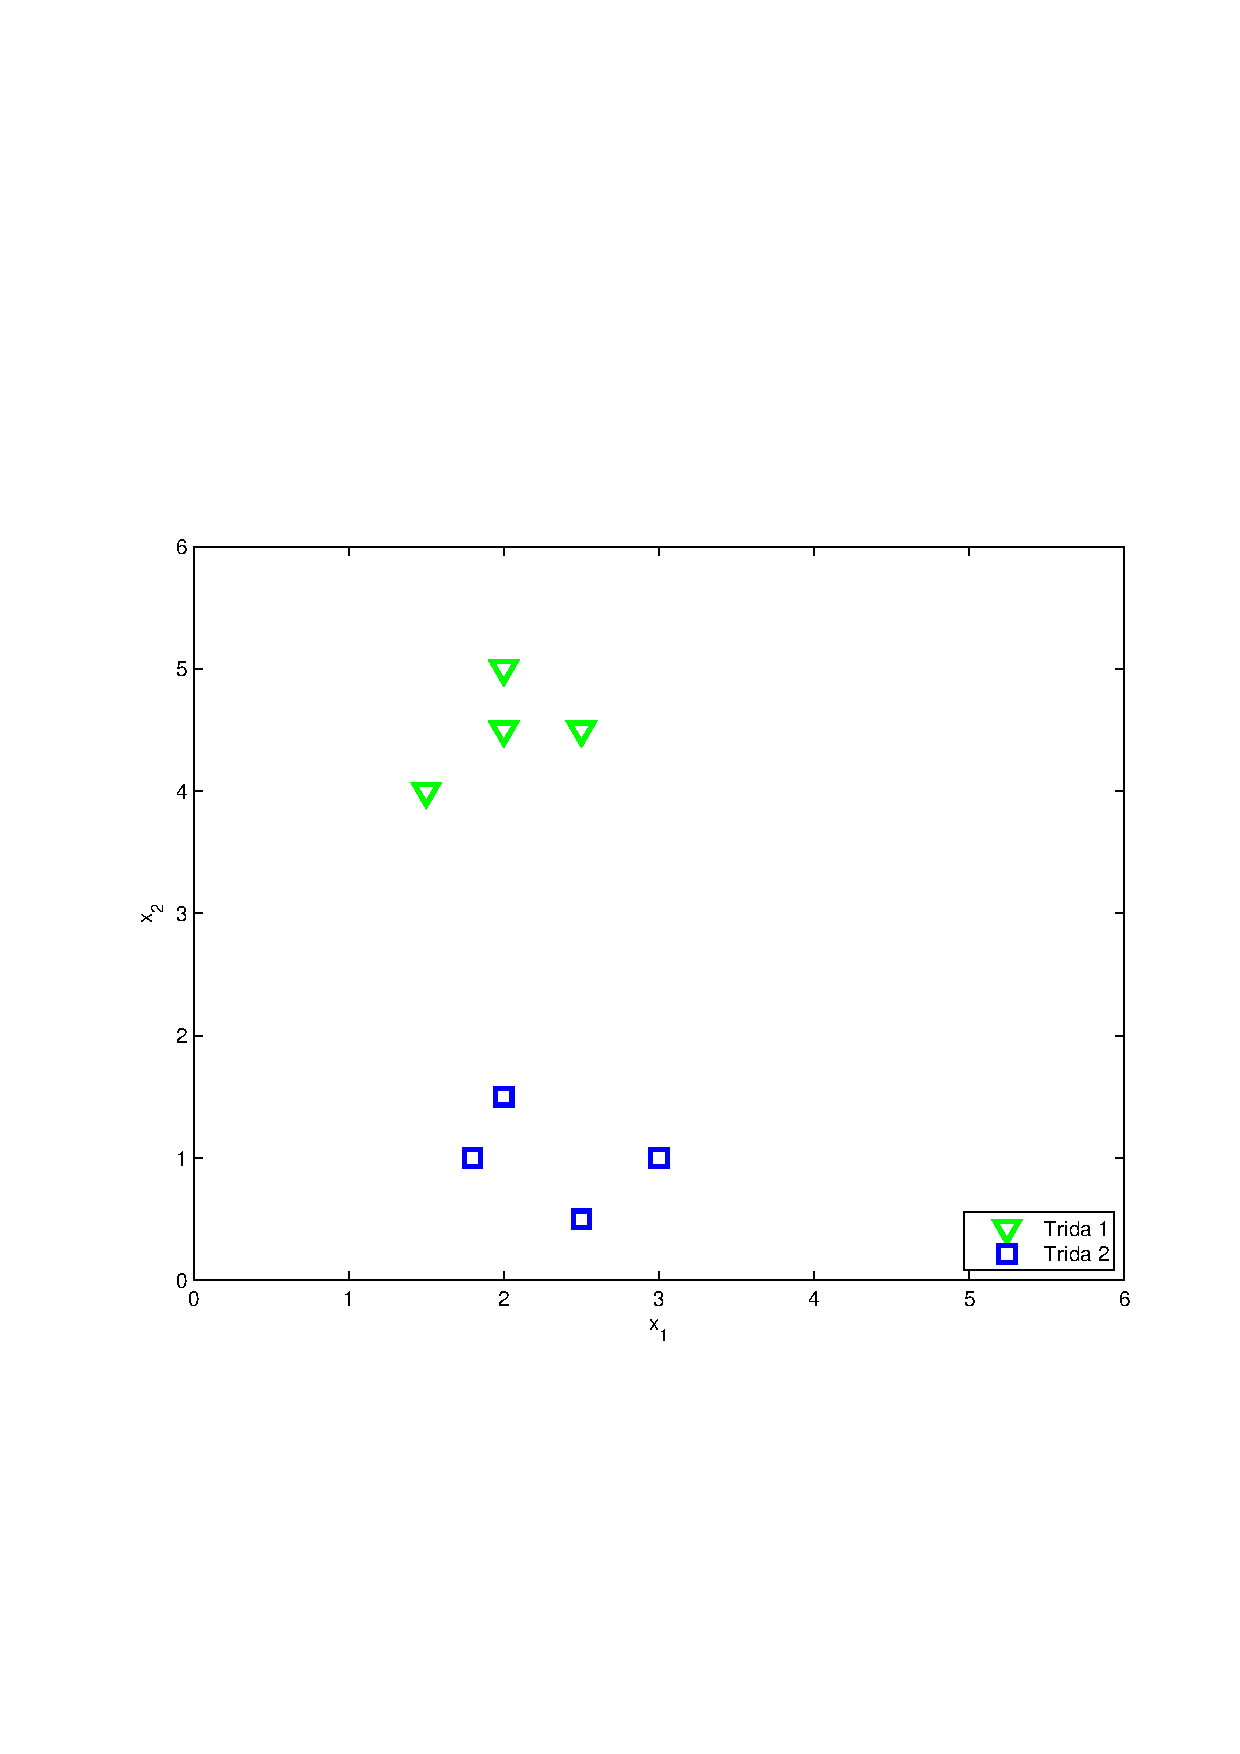
\includegraphics[width = \textwidth, trim = 2.5cm 7cm 2cm 9cm]{./Img/BinarniRegrese/oneVSallClassification/oneVSall_one.pdf}
  		\caption{Klasifikace do dvou tříd.}
		\label{fig:oneVSall_one}
	\end{minipage}%
	\hfill
	\begin{minipage}[b]{0.48\textwidth}
		%trim option's parameter order: left bottom right top
		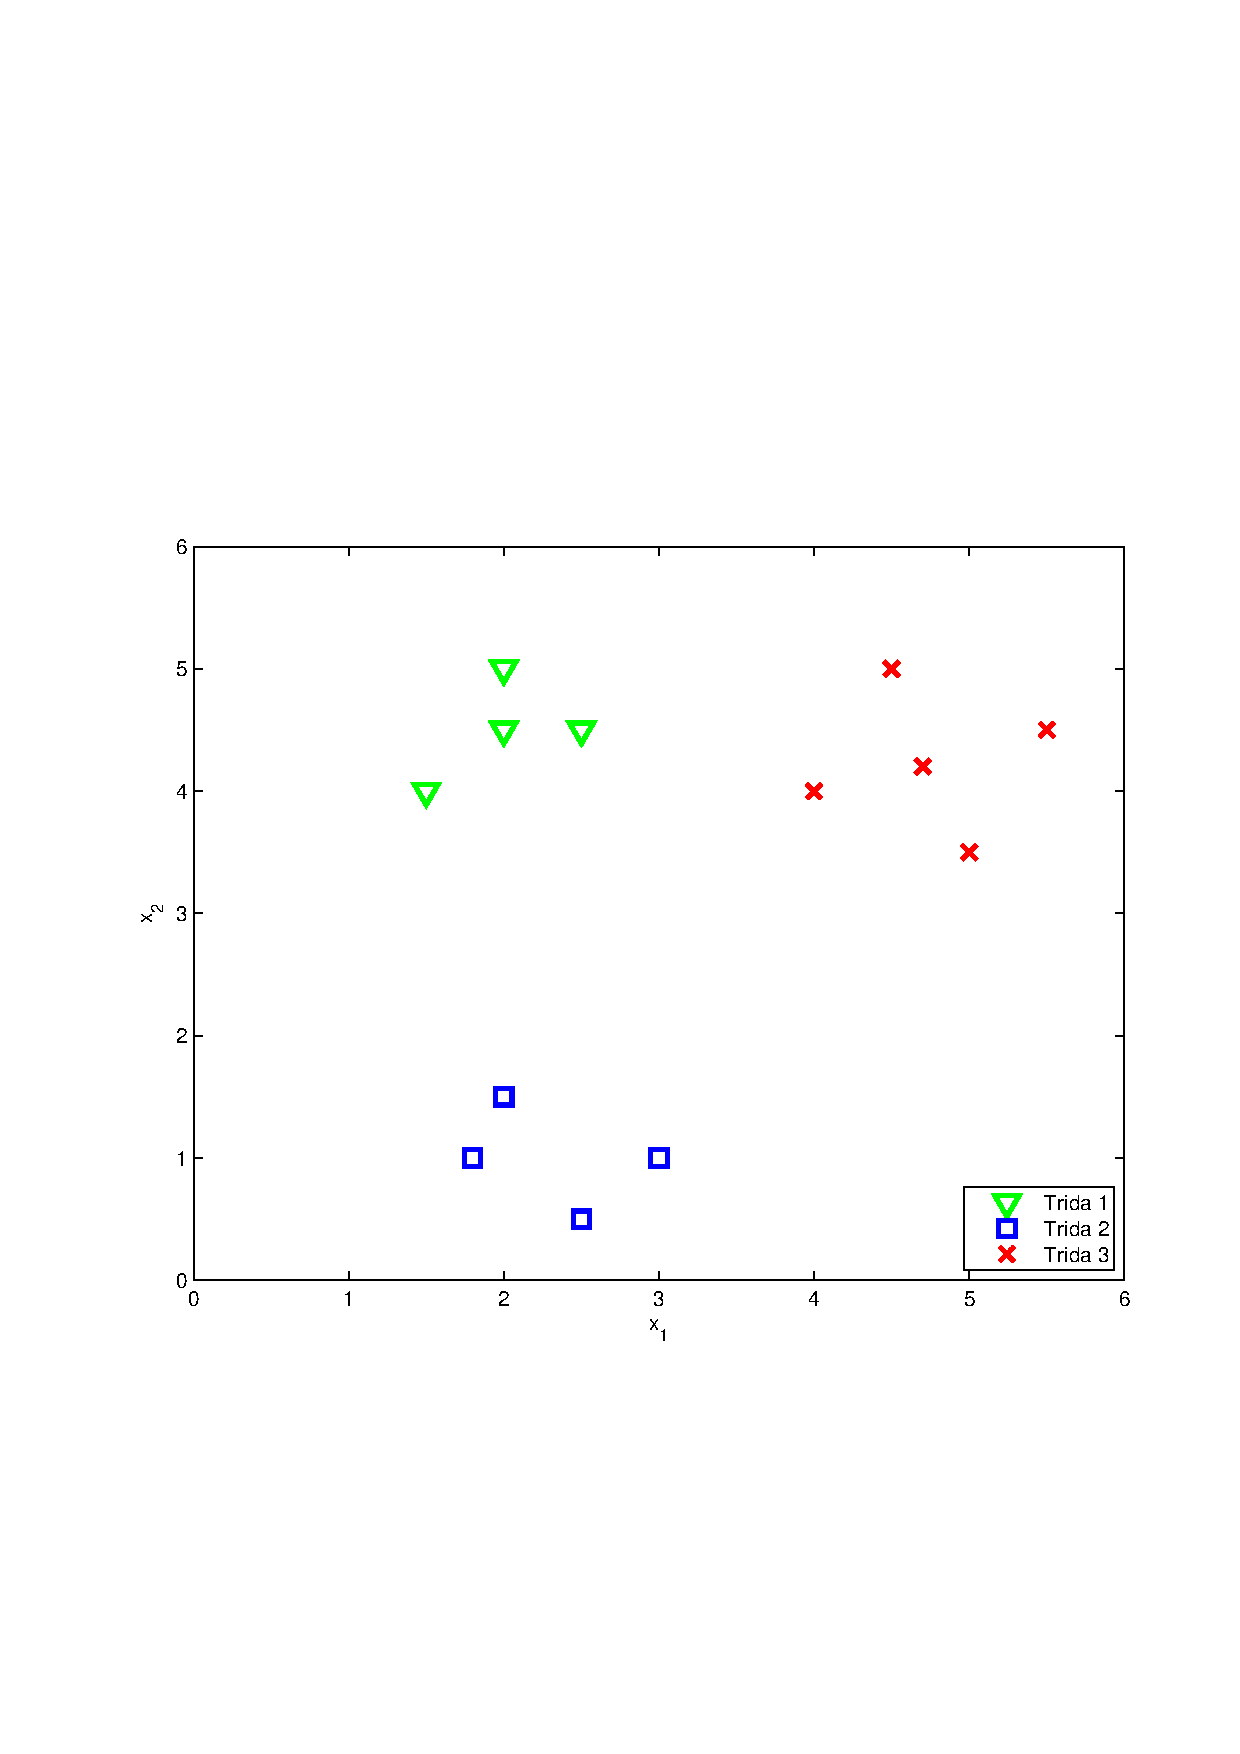
\includegraphics[width = \textwidth, trim = 2.5cm 7cm 2cm 9cm]{./Img/BinarniRegrese/oneVSallClassification/oneVSall_all.pdf}
  		\caption{Klasifikace do více tříd.}
		\label{fig:oneVSall_all}
	\end{minipage}%
\end{figure}}

\par{Z předešlých sekcí víme jak klasifikovat do dvou tříd. Nyní tento přístup použijeme při řešení problému klasifikace do více tříd. Na Obr. \ref{fig:oneVSall_all2} je znázorněno rozložení tříd a~následně na Obr.~\ref{fig:oneVSall_1} je ukázána klasifikace třídy~1 proti třídě, která je zkonstruována spojením všech ostatních tříd (v~našem případě tříd 2~a~3). Na dalších Obr.~\ref{fig:oneVSall_2} a~\ref{fig:oneVSall_3} jsou naznačeny zbylé kombinace.}Pro jednotlivé klasifikace je nutné vytvořit hypotézu
\begin{equation}
	h_{\bm{\Theta}}^{\left( i \right)} \left( \bm{x} \right), \quad i \in \{ 1,~2,~3\},
\end{equation}
která odpovídá pravděpodobnostem
\begin{equation}
	h_{\bm{\Theta}}^{\left( i \right)} \left( \bm{x} \right) = P \left( y = i| \bm{x} ; \bm{\Theta} \right).
\end{equation}}
\pagebreak

\begin{figure}[!ht]
	\centering
	\begin{minipage}[b]{0.48\textwidth}
  		%trim option's parameter order: left bottom right top
		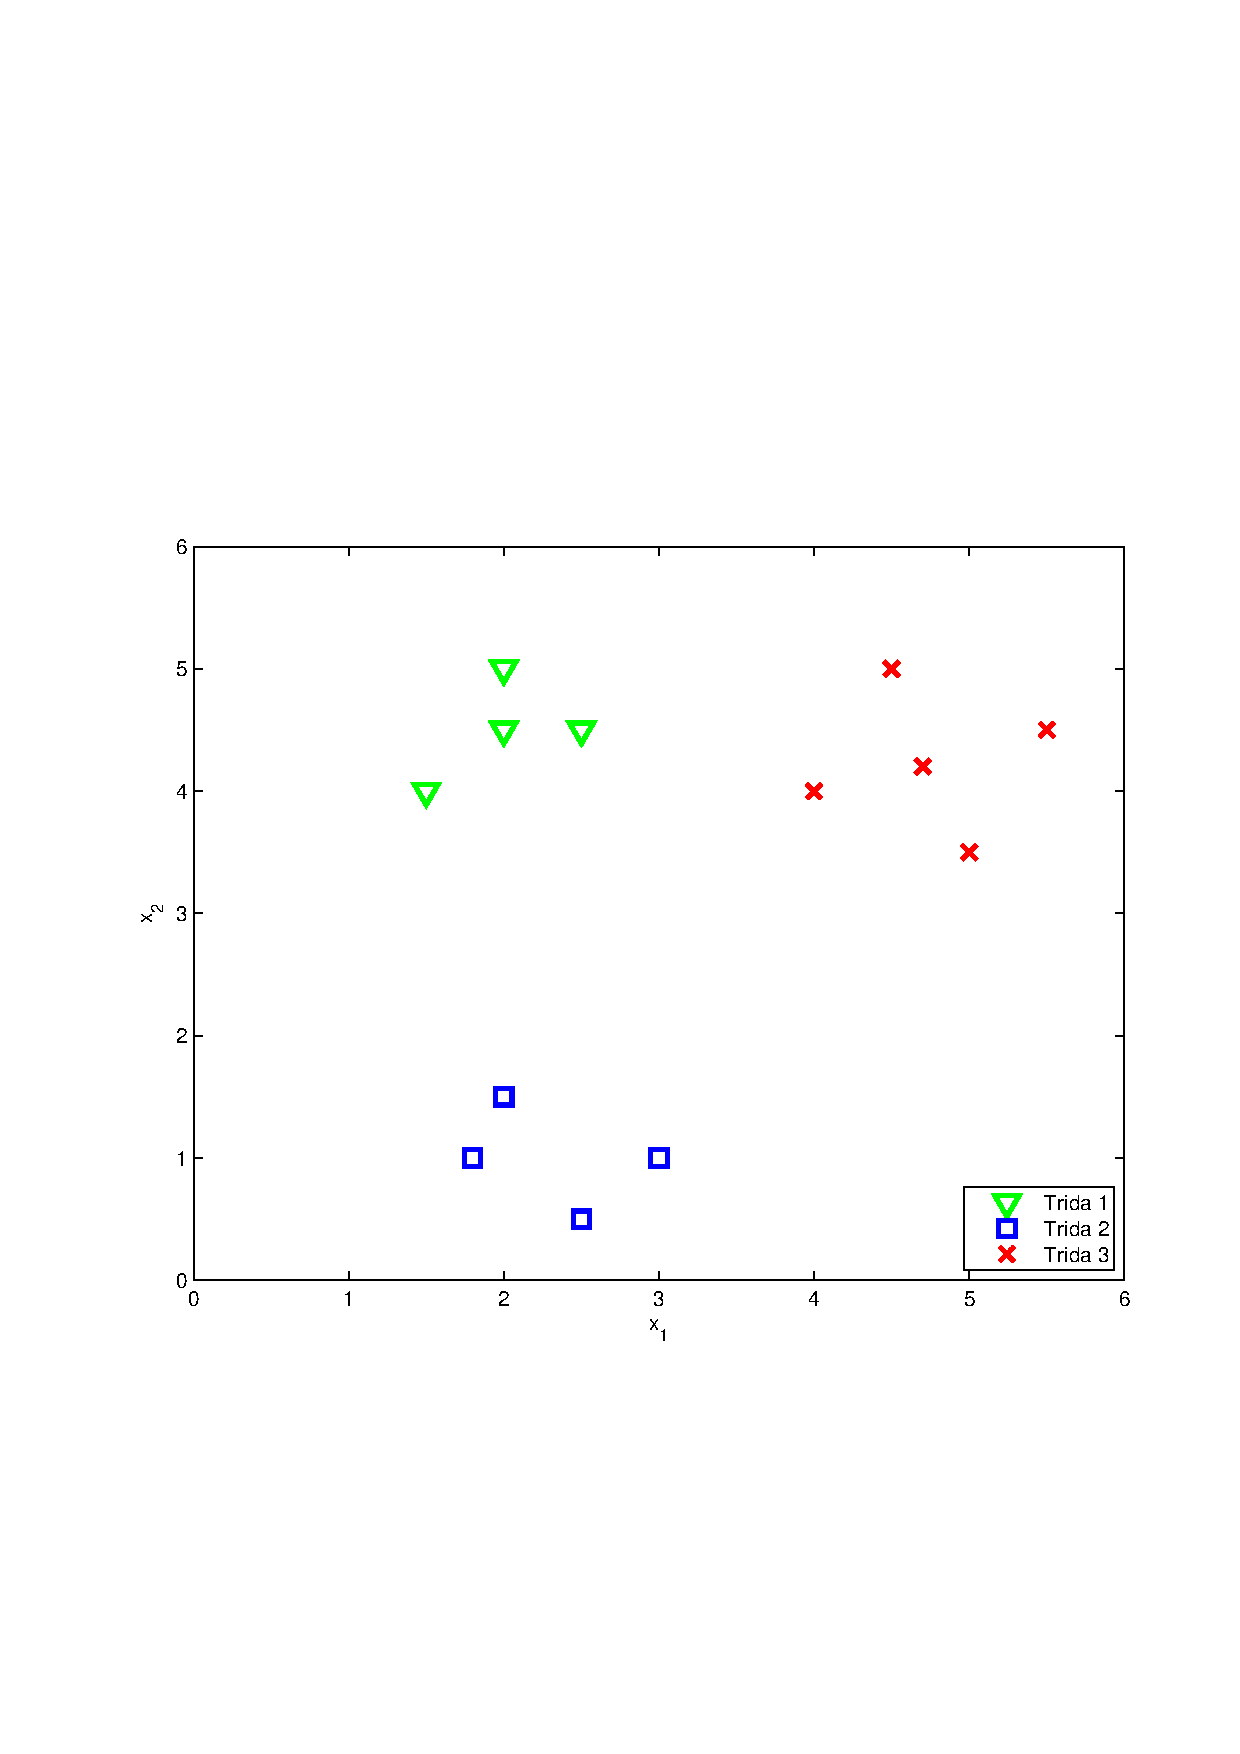
\includegraphics[width = \textwidth, trim = 2.5cm 7cm 2cm 9cm]{./Img/BinarniRegrese/oneVSallClassification/oneVSall_all.pdf}
  		\caption{Rozložení tříd $y = \{1,~2,~3\}$.}
		\label{fig:oneVSall_all2}
	\end{minipage}%
	\hfill
	\begin{minipage}[b]{0.48\textwidth}
		%trim option's parameter order: left bottom right top
		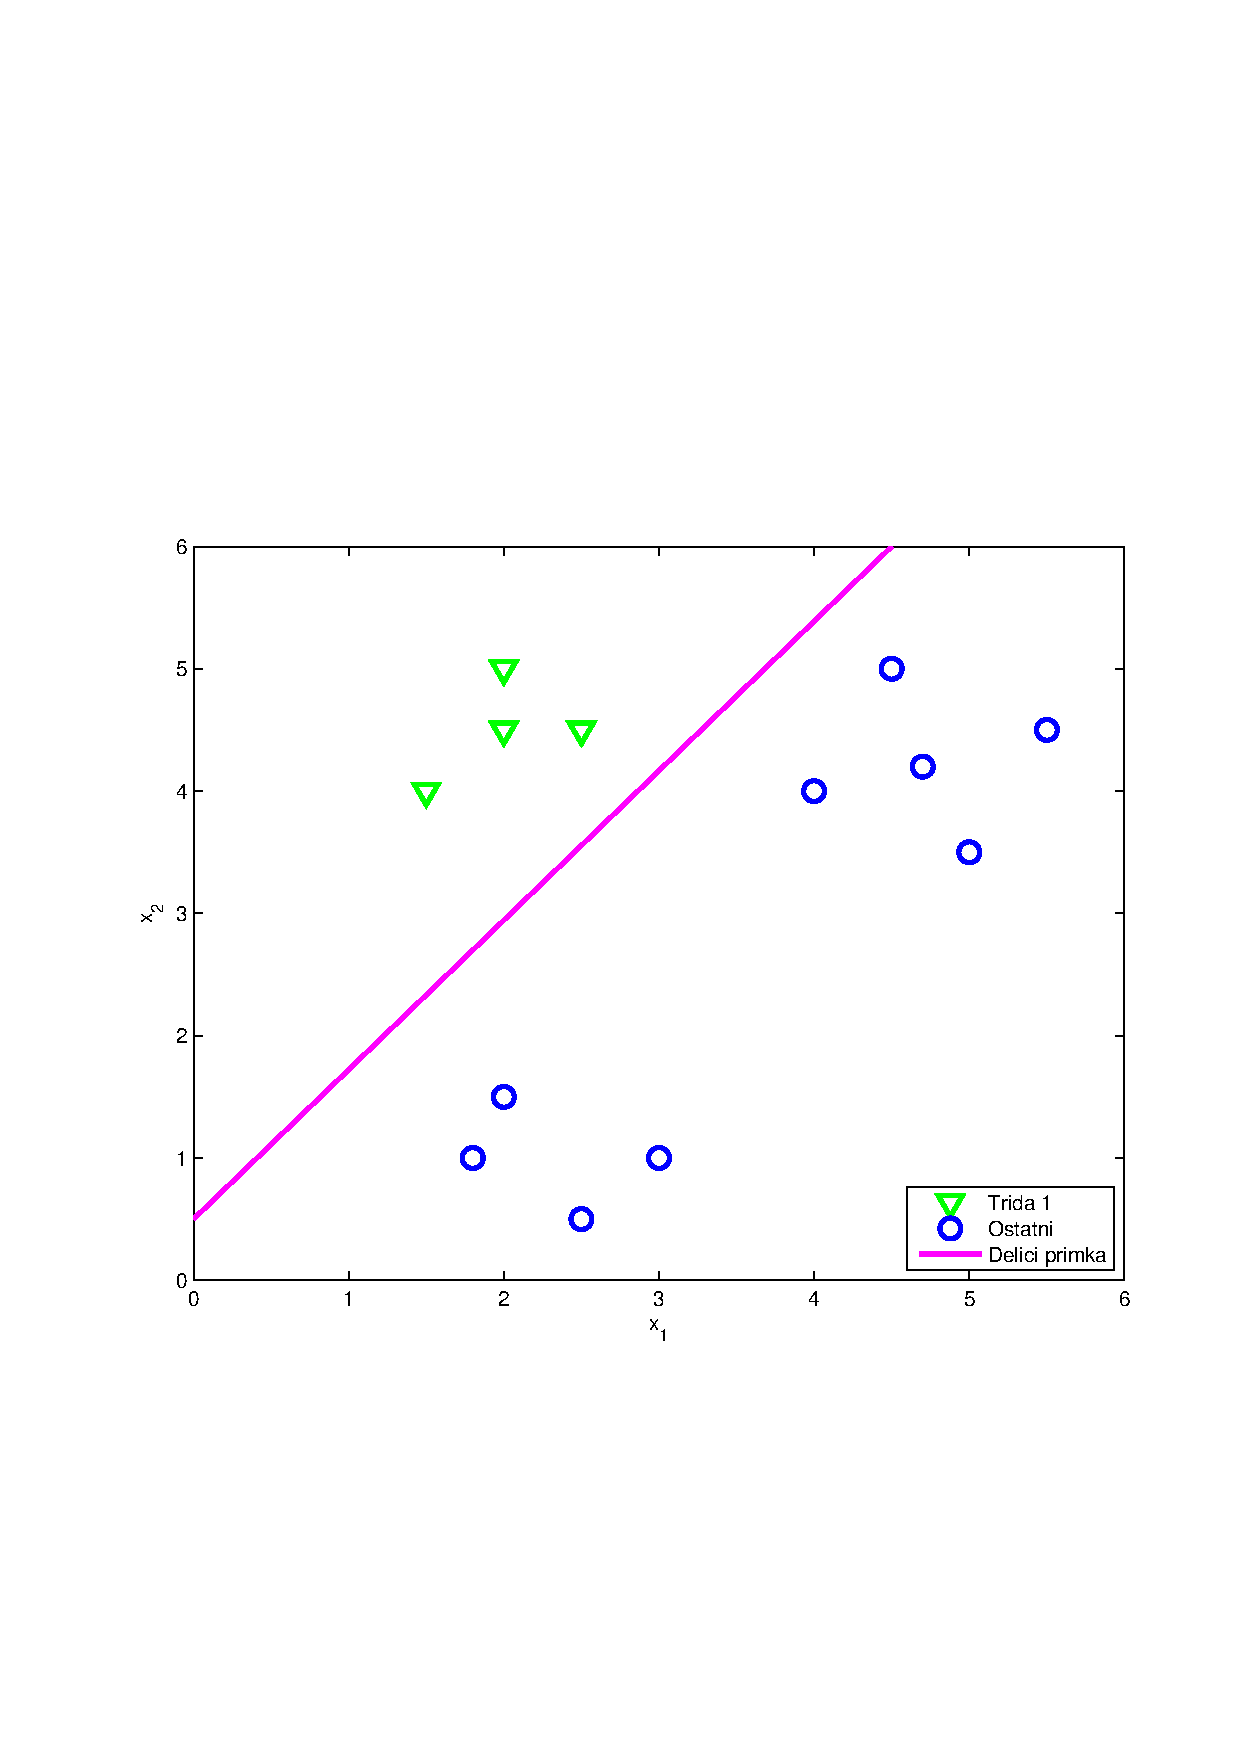
\includegraphics[width = \textwidth, trim = 2.5cm 7cm 2cm 9cm]{./Img/BinarniRegrese/oneVSallClassification/oneVSall_1.pdf}
  		\caption{Klasifikace třídy 1.}
		\label{fig:oneVSall_1}
	\end{minipage}%
\end{figure}
\begin{figure}[!ht]
	\centering
	\begin{minipage}[b]{0.48\textwidth}
  		%trim option's parameter order: left bottom right top
		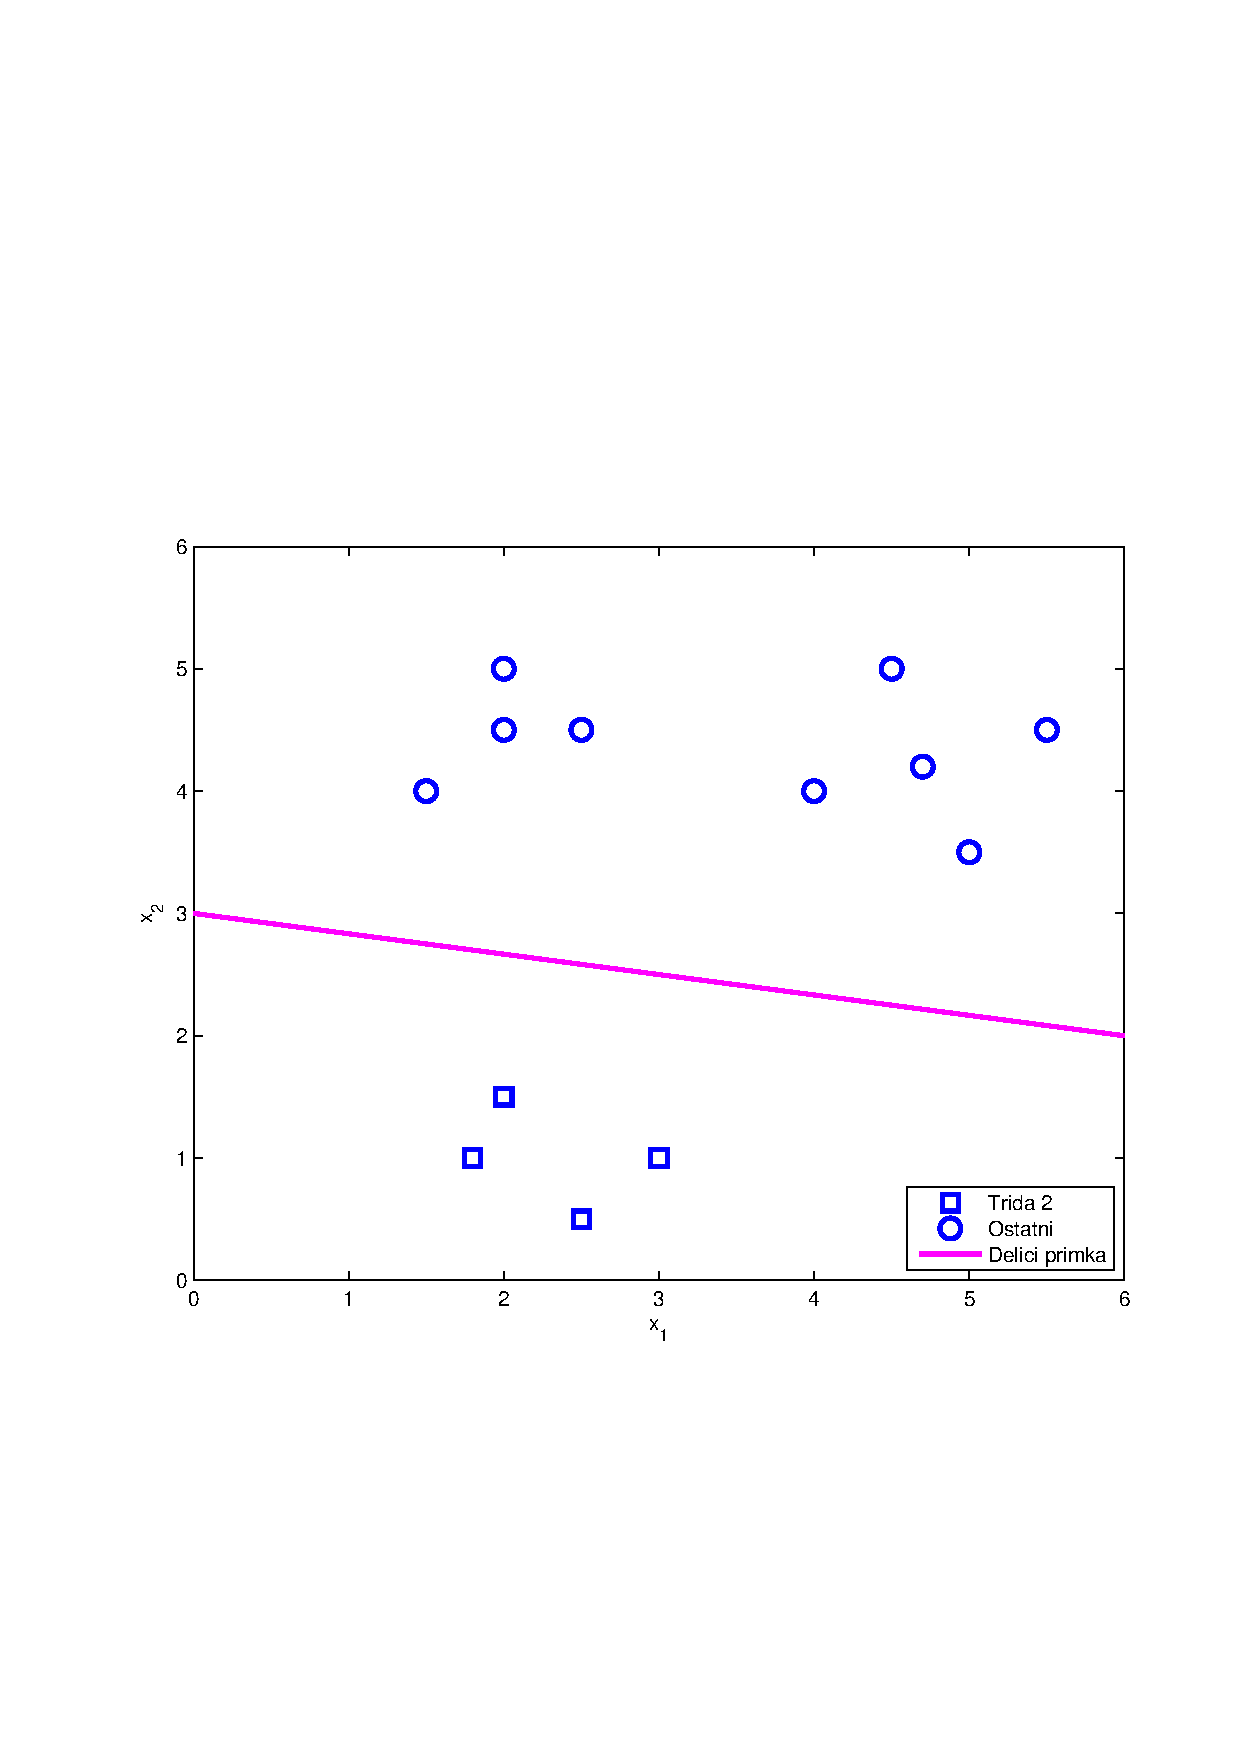
\includegraphics[width = \textwidth, trim = 2.5cm 7cm 2cm 9cm]{./Img/BinarniRegrese/oneVSallClassification/oneVSall_2.pdf}
  		\caption{Klasifikace třídy 2.}
		\label{fig:oneVSall_2}
	\end{minipage}%
	\hfill
	\begin{minipage}[b]{0.48\textwidth}
		%trim option's parameter order: left bottom right top
		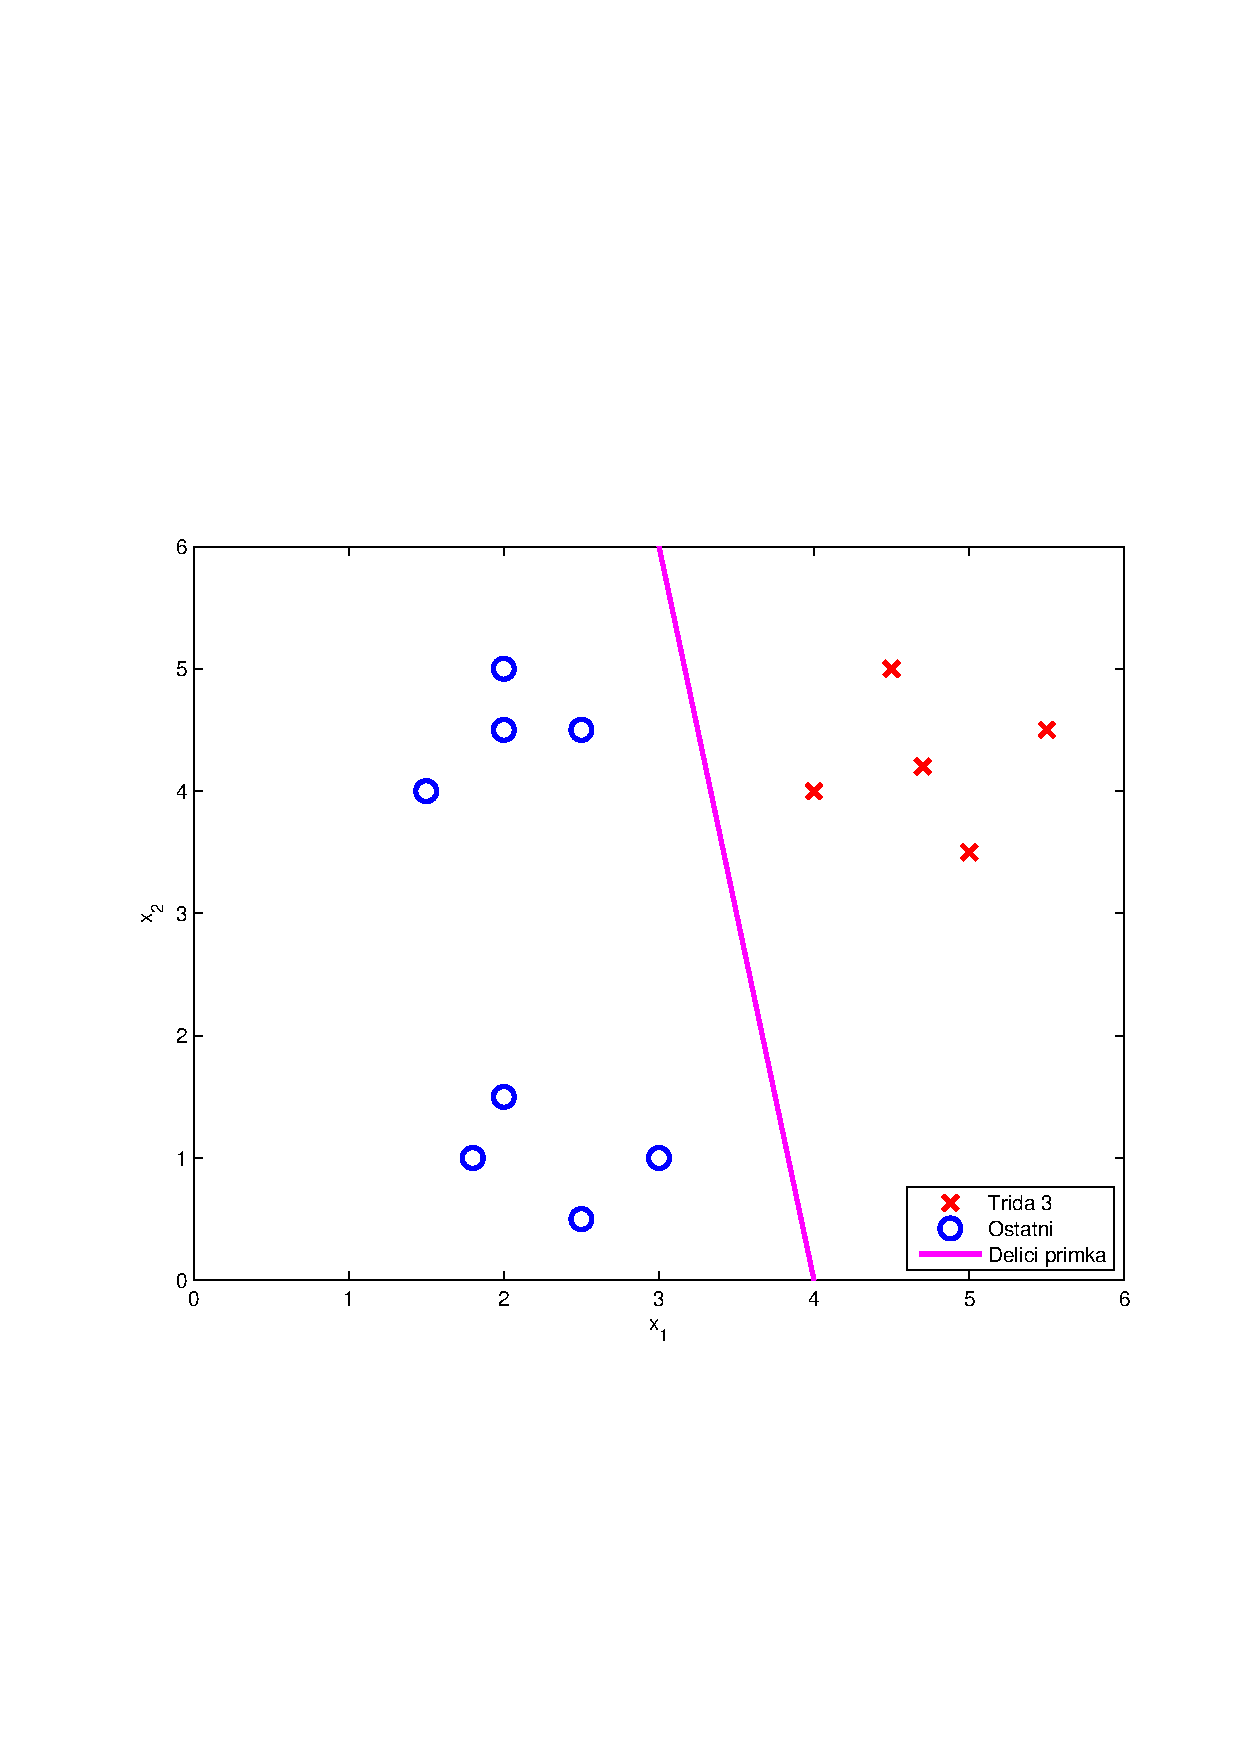
\includegraphics[width = \textwidth, trim = 2.5cm 7cm 2cm 9cm]{./Img/BinarniRegrese/oneVSallClassification/oneVSall_3.pdf}
  		\caption{Klasifikace třídy 3.}
		\label{fig:oneVSall_3}
	\end{minipage}%
\end{figure}

\subsubsection*{Shrnutí}
\par{Nejdříve je nutné natrénovat binární klasifikátory $h_{\bm{\Theta}}^{\left( i \right)} \left( \bm{x} \right)$ pro všechny třídy $i$ pro predikci pravděpodobnosti, že vzorek bude patřit do třídy $y = i$. Následně pro nový vstup $x$ klasifikovat podle všech hypotéz a vybrat takovou třídu $i$, která maximalizuje pravděpodobnost hypotézy
\begin{equation}
	 \max_{i} h_{\bm{\Theta}}^{\left( i \right)} \left( \bm{x} \right).
\end{equation}}


\newpage



















